\documentclass[journal,transmag]{IEEEtran}
\usepackage{flushend}

\usepackage{graphics}
\usepackage{graphicx}
\usepackage{epstopdf}
\usepackage{epsfig}

\usepackage[table]{xcolor}
\usepackage{ifpdf}
\usepackage{color}
\usepackage{multirow}
\usepackage{cite}

\usepackage[tight,footnotesize]{subfigure}



\definecolor{xy}{cmyk}{0,0.42,1,0}


% correct bad hyphenation here
\hyphenation{op-tical net-works semi-conduc-tor}


\begin{document}

\title{A Survey on Radio Resource Management in WLAN networks}

\author{\IEEEauthorblockN{Mohamed Amine Kafi\IEEEauthorrefmark{1},
Alexandre Mouradian\IEEEauthorrefmark{1},
V\'eronique V\`eque\IEEEauthorrefmark{1}}
\IEEEauthorblockA{\IEEEauthorrefmark{1}L2S, CentraleSUPELEC, Paris Sud University, FRANCE.}

\thanks{%Manuscript received December 1, 2012; revised September 17, 2014. 
Corresponding author: Mohamed Amine Kafi (email:kafiamine@gmail.com)}}



% The paper headers
\markboth{IEEE Surveys and Tutorials,~Vol.~xx, No.~xx, Avril~2018}%
{Shell \MakeLowercase{\textit{et al.}}: Bare Demo of IEEEtran.cls for Journals}


\IEEEtitleabstractindextext{%
\begin{abstract}

With the increasing use of Wireless local Area Networks (WLAN) in both home and industrial connections, RRM (Radio Resource Management) become mandatory in order to comply with existing and future high throughput applications requirements. A deep analysis of shortcomings and strengths of the existing radio resource management propositions is the first step to propose new ones or enhance the existing.   
In this study, we focus on the methods of client association to the Access Points proposed in the state-of-the-art WLAN works. As the default client connection method with the Access Points performed in IEEE 802.11 using the highest Signal Strength values presents throughput degradations, many works have being proposed to overcome this shortcoming. We have classified the proposed methods according to their centralised or distributed control. The centralised approach is further divided according to the fairness form that the controller tries to fulfill or according to QoS requirements. On the other hand, the distributed control is performed at the individual Access points or the joining clients, this is classified according to the used parameters, too. The use of SDN paradigm for controlling RRM is also introduced in our classifications. The deep discussion performed at the end of the study clarifies even more the different shortcomings and founds pillars that allow enhancements of RRM strategies.  


\end{abstract}

% Note that keywords are not normally used for peerreview papers.
\begin{IEEEkeywords}
Wireless LAN, 802.11, Controllers, Resource Control, intelligent networks, cellular radio, radio access networks, radio spectrum management, Access Point, Resource management, throughput. 
\end{IEEEkeywords}}

% make the title area
\maketitle

\IEEEdisplaynontitleabstractindextext
% \IEEEdisplaynontitleabstractindextext has no effect when using
% compsoc or transmag under a non-conference mode.

\IEEEpeerreviewmaketitle

\section{Introduction}
\IEEEPARstart{T}{}he Utilisation of WIFI is knowing more and more increase in the past years and will continue in the next ones, due to the explosion in the number of smart devices with the huge data traffic that results including smart-phones, laptops, tablets, terminal games and professional diagnostic suitcases. 
At the contrary of what one could imagine, the use of 3G and 4G (and will continue with 5G) has brought more use of WLAN rather than its decrease, as the sale and deployment of WLAN Access Points show in the market \cite{17why_Long_WIFI_Connect,14group_based_RRM}. Indeed, the availability of WIFI hotspots every where (indoor/ outdoor) makes it one of the preferable connection technologies for users. This is due to the cheap cost of WIFI to users and the number of Access Point available in residential habitation, commercial building, airports, malls, stadium...\cite{15Node_throughput_enhencement_wifi}. \\

The ease of using WLAN technology, at the same time of offering high bandwidth and taking users mobility into account make it very prevalent for Internet subscribers, companies and operators \cite{16AP_association_optimisation_fairness}. In addition, the operators perform offloading of their networks' traffic to the WLAN that presents less cost, more speed, robustness and reliability. In fact, one of the pillars for the 5G success is that many Radio Access Technologies (RAT), as WLAN, will be integrated in the aim to enhance users QoE (Quality of Experience) \cite{17QOS_AP_selection}. \\

In practice use, the architecture of a WIFI network could be as simple as a single Access Point that serves many wireless devices under its coverage, like in an apartment, to a deep complex architecture in which organised/ individual Access Points cohabit in industrial or citizens network scenarios covering the whole network in a manner similar to that of cellular networks, where the coverage of each Access Point constructs a cell. 
Indeed, in public and commercial areas many Access Points are present and offer free access to the Internet for the users, after a security registration form, in order to check the e-mails and browse the web while walking thorough the commercial zones corridors \cite{16VALI_SDN}. Some of these hotspots belong to the same authority like the organisers in the malls or airports, and other ones are individual like that of the shops. The aim of using shops' individual Access Points is to enhance users access and QoS by offering fast service like that of visualizing shops offers and videos while staying in coffee shops. 

The Access Points are related on the wired backbone, through the access router for example, that is supposed generally having a high performance, while that of the wireless part is supposed to be the bottleneck of bandwidth. The users could roam from one Access Point to another as they walk and possible disconnections are very frequent. During the communications, uplink flows resulting from the users traffic thorough the network or downlink flows from the network thorough the users could be present, with downlink dominating flows as in cases of video streaming or email checking, or also web browsing \cite{05DIRAC}.    

The diameter of cells changes according to the coverage in indoor and outdoor scenarios and chovochement between cells is mandatory in order to avoid disconnections of the users while changing the cells \cite{15fuzzy_load_balancing_802.11}. \\

The dense and mesh architecture of WLAN networks that gives it the robustness in large networks size is at the same time the cause of its shortcoming and lack of throughput. In fact, the non organisation of Access Points resources leads to severe throughput degradation due to the high interference levels seen in the intra and inter cells \cite{15Node_throughput_enhencement_wifi}.
This could happen when a user of a given Access Point is communicating, and other individual Access Points being in the same sensing or receiving vicinity communicate at the same time on the same channel with their clients, which leads to collisions and interfering communications. This behaviour results to the loss or corruption of the sent packets and therefore the individual and aggregated network throughput will decrease significantly. The use of the same channel by these Access Points could be due to the lack of orthogonal channels, or to simply the lack of organisation between individual Access Points \cite{16AP_association_optimisation_fairness}. \\

As users distribution is not uniform \cite{14AP_association_multirate_WLAN} nor their capacity demand related to the used application \cite{17QOS_AP_selection}, associating the new arriving clients as the standard 802.11 policy according to the strongest signal Access Point could be a bad choice \cite{14optimalAP_INFOCOM}. In fact, the strongest signal Access Point could use the same channel as some neighboring Access Points leading to high interference, while less power signal Access Point is existing, with other unique channel use. On the other hand, the interference avoidance method largely used for WLAN communications at the MAC Level, namely the DCF (Distributed Coordination Function) could not resolve completely the interference problem, especially in the case of hidden terminals where users exist in the vicinity of two Access Points that do not hear from each other \cite{04Intelligent_resource_management}.

This same standard association causes also that some Access Points become overloaded with the increase of users number and constitute the bottleneck of the whole network \cite{14AP_association_multirate_WLAN} with users given low QoS, while other Access Points having little clients or low capacity demand and so lightweight load keep unused because of their low signal strength. Such scenarios are very frequent in boarding lounges at the airports and train stations or concentrated tables in a restaurant, and the corresponding users see them selves with mediocre offered capacity and unnecessarily long delays \cite{15Node_throughput_enhencement_wifi,15OpenSDWN_home_entreprise_WIFI,14online_AP_association_80211n,10Assesment_EDCA_real_time,16Indoor_spatial_reuse_adaptive_antenna}. 
The performance degradation in this case is due to that the users must share the airtime served by the Access Point and the bandwidth is indeed divided \cite{04Intelligent_resource_management}. Furthermore, the effective airtime should be shared also with the neighboring Access Points clients that use the same channel, and are in the sensing vicinity \cite{11user_centric_management_WLAN}. This results on bandwidth unfairness between the users of the whole network \cite{16AP_association_optimisation_fairness}, when compared to less loaded Access Points.

Even more, in such environment, users could be obliged to use different bitrates to surmount the losses, where stations distant from Access Points or with thick obstacles use low bitrates compared to closest stations or that without obstacles \cite{15time_fairness_MAC}. When a user uses a low rate transmission, the other connected users on the same Access Point will see their effective rates reduced to less than the slowest rate user (perceived individually), as they share the bandwidth equally. This is explained by the fact that the slower users occupy the channel for longer periods to have the same bandwidth as the faster ones. \cite{16AP_association_optimisation_fairness}.

But even with the existence of some commercial solutions used for enterprise or malls scenarios for network resource management through controllers, this last keeps proprietary and does not adapt with the low cost large used devices, nor Access Points used by residential or shops, especially with the paradigm BYOD (Bring Your Own Device) in which lambda users in the malls and the airport would like see their performance enhanced without any change in drivers nor taking special measures \cite{15OpenSDWN_home_entreprise_WIFI,17QOS_AP_selection}. \\

%==============================================
\begin{figure}[t]
\centering
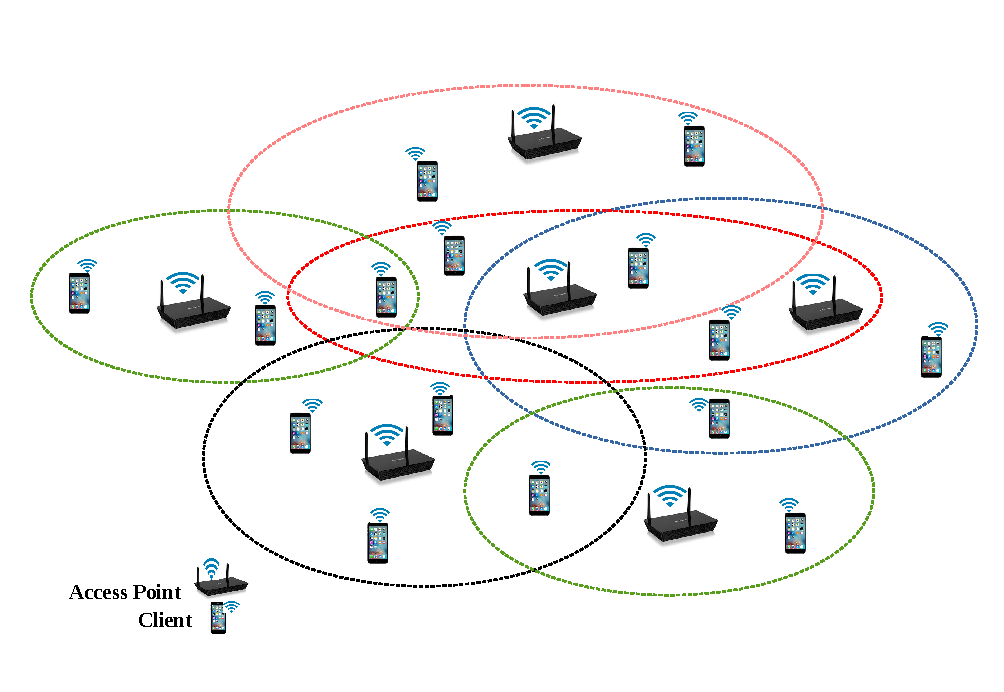
\includegraphics[width=9cm]{Figures/Dense_WLAN.pdf}
\caption{Multi cell WLAN Network}
\label{multi_cell_WLAN}
\end{figure}
%==============================================

The ultimate solution for radio ressource management is to monitor the available capacity resources and intelligently sharing them in a manner that loads-balance the Access Points charge and decreases the interference between adjacent ones by intelligent channel attribution and users associations. Taking into account the dynamic change in the users resource demands, related generally to the application and priority of users, will enhance deeply the offered resources with the required fairness methods \cite{16VALI_SDN}. The problem of roaming the users in a transparent manner that avoids disconnections is very important and should not be triggered only according to signal strength but for also other parameters related to the individual or aggregated QoS \cite{14optimalAP_INFOCOM,14Odin:Programmatic_Orchestration_WiFi}. Using the SDN (Software Defined Networking) paradigm, where the different performance parameters are changed as services according to the controller orders is very important, as it allows dynamic definition of system requirements without changing hardware configuration \cite{14Odin:Programmatic_Orchestration_WiFi}. \\
Despite the existence of many propositions in literature in order to enhance the radio ressource management in WLAN scenarios generally and client Access Points Associations especially, but to the best of our knowledge there is no review studies proposed to clarify and classify the aim and families of works in this field. In the following study we focus our selves on the client Access Point works and try to show the pros and cons of the proposed works and open tracks in which enhancements should be performed to fill in the performance gaps. \\

The remainder of the paper will be organised as follows. The section \ref{RRM_WLAN} describes the pertinent parts of the radio ressource management for WLAN. While the section \ref{Taxonomies} presents the classifications that we propose and the basic elements used in these taxonomies.
In section \ref{evaluation parameters} we present briefly the parameters used to evaluate the state-of-the art works performance. After that, the section \ref{802.11 principe} explains the standard association under 802.11 behaviour and some standardisation groups related to the association. 
We analyse and discuss many points related to the client Access Points methodologies in section \ref{Discussion}. Finally, we conclude and give a summarization of the study in section \ref{Conclusion}.

%==============================================
\begin{figure}[t]
\centering
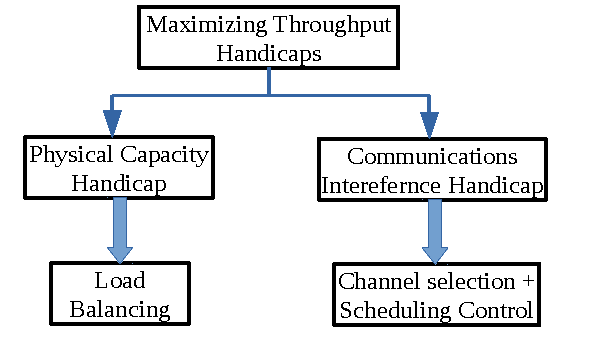
\includegraphics[width=8cm]{Figures/throughput_handicaps.pdf}
\caption{Throughput Maximisation Handicaps}
\label{throughput_handicaps}
\end{figure}
%==============================================

\section{Radio Ressource Management} (me)
\label{RRM_WLAN}

The dense deployment of WLAN become more and more frequent due to the success that knows and the increase in the applications diversity and requirements. In such environment, many APs are present in an overlapping manner constructing a multi cell network that obliges a deep organisation in order to increase the throughput through cells coordination, Fig.\ref{multi_cell_WLAN} shows a possible architecture of such network. In fact, the diversity of applications and their exigency in rate lead to continuous increase in throughput need. On the other hand, two handicaps should be fulfilled to track this need (see Fig.\ref{throughput_handicaps}). The first point is the physical rate capacity limitation of each AP that imposes organisation in the associations in order to load balance the charge. The second point is to decrease interference as possible to avoid communication failure. These two aspects open three main fields for radio resource management in WLAN. Namely, how to associate the clients with the Access Points in order to optimise physical capacity use. The second field concerns how to select the channels, as the dense deployment of APs constructs a multi cell network for which interfering channels should be monitored to allow spatial reuse as possible. Also the third field is to schedule communications in order to avoid interference in the intra and inter cells. A fourth field that could be used in conjunction with the three aforementioned fields is the power control of communications that helps to put in practice the other Radio resource management aspects. \\
The summary of the resource optimisation is that before the use of a multi-cell WLAN, the different Access Points should select their channels to communicate. The clients afterthat associate to the APs according to a given parameter(s). The third step is that the communications are scheduled in a given manner (coordinated or randomised). As the research works that will be presented in the following sections show, a combination of the previous steps could be performed for optimisation purposes, like the channel selection and client-AP association at the same time (centralised \cite{06client_channel_WLAN}, distributed \cite{07measurment_self_WIFI}), or the three ressource managements steps channel selection, client-Access Point association and communications schedule as in \cite{14proportional_fairness_distributed_multiband} (in distributed manner). In Fig.\ref{fig:RRM} the previous research fields are depicted, while the following sections describe in more details each part of RRM.  

\subsection{Channel selection strategies for APs} (me)
In a large WLAN network, a single Access Point could not cover the whole network as the emission power is limited. On the other hand with the increasing number of users, the Access Point bandwidth capacity become insufficient to answer all the users bandwidth demand. For that, putting many neighboring Access Points is necessary. In practice, many neighboring Access Points coexist to cover the large network but this chauvochement between Access Points makes a problem related to the number of orthogonal radio channels that is limited and does not allow to assign them in a conflict free graph manner \cite{15channel_selection_dynamics_dense_wifi} and reusing the same channel is so mandatory. 
From another angle, the fact of using WLAN in indoor environment, propagation models are hard to predict. For that, network administrators use many methods in order to choose the appropriate channels attribution after conducting Radio Frequency (RF) site surveys \cite{06client_channel_WLAN}. But even with this initial affectation, Access Points should monitor their surrounding, with possible dynamic obstacles and especially dynamic traffic that push to change this channel affectation. 

In literature many works interest on the channel assignment problem \cite{15COAP,13outsourcing_AP_cloud_API,11PIE_sky,16SDN_based_channel_assignement,16centralised_wifi_manegement,15channel_selection_dynamics_dense_wifi,05weighted_coloring_channel_assignement_WLAN,05frequancy_allocation_graph_coloring,06self_managed_distributed_channel_selection,07Traffic_channel_assignment_WLAN,07distributed_channel_assignement_multiradio_mesh,14channel_selection_regression,16CCI_queuing_model,15WI_FM,09adjacent_channel_interference_allocation,08channel_assignement_SIR_WLAN,13adaptive_proportional_fairness}. Some of these works try to propose centralised approaches in which a controller fixes the used channel for each Access Point according to many parameters \cite{15COAP,13outsourcing_AP_cloud_API,11PIE_sky,16SDN_based_channel_assignement,16centralised_wifi_manegement,15channel_selection_dynamics_dense_wifi}. In other works, distributed methods were proposed in which the concerned Access Point chooses its channel, after exchanging information of its surrounding \cite{05weighted_coloring_channel_assignement_WLAN,05frequancy_allocation_graph_coloring,06self_managed_distributed_channel_selection,07Traffic_channel_assignment_WLAN,07distributed_channel_assignement_multiradio_mesh,14channel_selection_regression}. Deeper classification of this research field is planned for future study. 

\subsection{Association of clients to Access Points (me)}
In order to use the WLAN resources, each client should associate to an Access Point before starting the communication. The default association of clients with the APs performs using the highest signal strength method. This strategy is not the best in a multi cell network environment where the AP with the highest signal strength could be high loaded while other less strength APs could offer higher throughput. Choosing also other APs rather than the highest signal based one could be due to less interference in the other candidate APs or for load balancing purposes like fairness between different clients. Choosing the best AP to which associate a client could be performed in a centralised manner \cite{10approximate_optimisation_proportional,14AP_association_multirate_WLAN,15Demand_aware_load_balance_WLAN,16throughput_optimisation_association_bandwidth,14optimalAP_INFOCOM,12Network_cooperation_AP_association,11proportional_fairness_power_control,16AP_association_optimisation_fairness,07optimal_association_MSWIM,15AP_association_MIMO,08AP_assignement_algorithms,08proportional_fairness_multiRate_LAN,06proportional_fairness_3G_networks,04Fairness_load_balancing_WLAN,07fairness_load_balancing_LAN,17QOS_AP_selection,16centralised_framework_AP_selection_fittingness_factor,10Dyson,08Design_high_wifi_entreprise,06client_channel_WLAN,06practical_queue_based_AP_association,13sociality_aware_AP_slection,15fuzzy_load_balancing_802.11,05optimal_AP_selection,05optimal_association_stations,08load_balancing_QOS,09achieving_effeciency_fairness_vehicular,09dynamic_association_load_balancing,10game_load_balancing_association,10joint_bandwidth_association,10dynamic_load_balancing_industrial,14load_handoff_SDN,15load_performance_enhancement} where a controller has a global view of all the network, through the information sent by the APs under its responsibility, in addition to optionally other information from the clients themselves. The second option is to perform the association by a distributed decision \cite{01dynamic_loadBalanceWLAN,04decentralised_AP_selection_architecture,04decentralised_AP_selection_robusteness,05facilitating_AP_selection,05self_organisation_interefring_WLAN,06AP_slection_strategy_IEEE11_E,06need_cross_layer_AP_selection_algo,07measurment_self_WIFI,07Multihoming_users_AP_population_game,07AP_selection_large_scale_WLAN,08available_bandwidth_based_AP_association,08QOS_AP_selection_pre_load_balancing,08association_game,10distributed_AP_selection_no_regret,10Practical_AP_Association,10Virtual_AP,10indoor_spatial_reuse_directionnal_antenna,11Multichannel_AP_seamless_handoff,11contention_traffic_load_aware_association,11ditributed_resource_proportional_fairness,11AP_selection_congentive_radio,11channel_Association_game,11distributed_AP_selection_power,11stability_fairness_APselection_game,11AP_association_channel_switching,11supervised_learning_congnetive_AP_selection,11user_centric_management_WLAN,12AP_association_80211n,12neural_network_congetive_AP_selection,13SAW,13SAW2,13optimising_association_miliwave,13smartAssoc,14online_AP_association_80211n,14strategy_diffrentiated_AP_selection_application,13AP_selection_qos_requirement_variable_channel,13cross_layer_AP_selection_distributed,14proportional_fairness_distributed_multiband,14throughput_optimisation_AP_association_interefrence,14AP_selection_game_mobile_users,15dynamic_AP_association_SDN,15AP_selection_game_correlated_equilibrium,15AP_selection_coordination,15optimisingAP_association_Mili_wave,15AP_association_CCA,16improving_AP_association_channel_utilisation_adaptive_probing,16channel_measurment_AP_selection,17decentralised_AP_selection,17AP_selection_adaptive_CCAT,17why_Long_WIFI_Connect,16Indoor_spatial_reuse_adaptive_antenna,16SDR_directionnal_channel,15AP_selection_multirate,15online_channel_select_user_association,14utility_based_AP_selection_QOE,13trigger_based_dynamic_load_balance_virtualised_interface,12smart_association_maw_flow,11localised_AP_selection,11multi_rate_AP_selection,10trafic_aware_decentralised_AP_selection,10potential_throughput_AP_selection,10CLASS_association_Mesh,09client_driven_load_balancing,09traffic_balancing_dynamic_AP_selection,09method_AP_selection,09throughput_measurment_AP_selection,08dynamic_load_balance_mobile_users,07AP_selection_improving_througput_fairness,07adaptive_AP_selection,07AP_selection_maximising_throughput,06effective_AP_selection_load_balancing,06AP_selection,08new_AP_selection,08interference_aware_decentralised_AP_selection} even by the client itself, or by the APs in its vicinity, without coming back to a central controller. 
Centralised approaches need more overhead and collaboration but have a global view of the network resources and could result on a more throughput maximisation and fairness \cite{17QOS_AP_selection}. However, due to network size scale and parameters handling, this approach could not be practical which pushes the use of distributed associations at the level of the clients themselves (for example \cite{14AP_selection_game_mobile_users} or Access Points individually (for example \cite{14throughput_optimisation_AP_association_interefrence}). In this case, the overhead is less than that of the centralised approaches but the view of the resources could be local and not optimised as in the centralised association. \\

In addition to the centralised or distributed Access Point selection. The aim to be maximised could differ from an application to another one according to the utility function to optimise \cite{17QOS_AP_selection}. The most important parameter that state-of-the art works present is the throughput. The throughput of individual users is handled specially with the distributed strategies based on the clients themselves, while packet loss rate could also be concerned. With the centralised approaches, the whole network throughput is object of maximisation. Ensuring a certain form of fairness, or prioritisation between the clients is also considered in centralised approaches. This is also envisaged with the distributed strategies where the individual Access Points monitor their sub networks. The energy handling could be also optimised through power control.\\    
Another important parameter that some state of the art works have taken into consideration is the resource demand of the clients \cite{07optimal_association_MSWIM,16throughput_optimisation_association_bandwidth} rather than a partition of ressources according to the links characteristics or coarse load balancing or also strict fairness. \\
Apart from the first association of a client with a given Access Point according to the previous parameters, the change in the parameters during the application lifetime could trigger re-association with other Access Points. This same operation is triggered by mobility (that leads to change in signal strength) in standard association, which is also named \textit{roaming}. Performing the re-association in a transparent manner, that doesn't lead to loss of packet information nor to high delay is for great importance for the success of the application. \\
Another parameter that should be tackled by any association different from the standard IEEE802.11 is the level of software change, namely at the Access Point level or at the client level. In centralised association, the change could be needed only at the AP level, if the client does not communicate extra information than that sent by the standard, and needed on the client level in addition to the AP if the client should communicate vital information (like its interference vicinity). In the distributed association, decided by the client, the change is performed at the client level. 

\subsection{Enhancing throughput by scheduling communications} (me)
The aim of scheduling users communications is to surmount the problem of DCF that attributes the same long term bandwidth to the clients associated with the same Access Point when having dissimilar physical rates between its clients. Also scheduling communications of the neighboring Access Points clients allows decreasing interference between their communications. Scheduling could consist to changing collision window size according to different parameters, while ensuring some kind of fairness between the users. In literature, many works interest on this research field \cite{15upstream_schedule_wifi,10splitAP_flexible_sharing,10throughput_performance_varible_load,07proportional_fairness_throughput,13proportional_fairness_channel_access,13centralised_schedule_WLAN,09CENTAUR,06MIFI_fairness_multipel_AP,14group_based_RRM,05IdleSense,06Optimal_CWmin_Selection,14leverage_SDN_openFlow_entreprise_WLAN,15time_fairness_MAC,12Maximising_throughput_time_fairness,05proportional_fairness_WLAN,04time_based_fairness_multirate_WLAN,14interference_fairness_infocom,16rigourous_practical_proportional_fair_AP,11Rigourous_proportional_fairness} and could be divided into many classes according the type of targeted fairness, in addition of performing the schedule in a centralised or distributed manner.   

\subsection{Power control for enhancing throughput} (me)
The aim of using power control is to change the coverage of the Access Points in order to decrease interference levels between the neighboring Access Points by decreasing the emission power. Also, power control could be used for eliminating coverage holes by increasing power emission of some Access Points. So, by performing the Power control we choose the correct power emission to enhance ressources use in such cases \cite{08power_control_fairness_optimisation,07interference_mitigation_power_control,14Gap_free_load_balancing_cell_breathing,08cooperative_load_balancing_cell_breating,09Cell_breathing_Load_balancing_WLAN,07Cell_Breathing}.

For the remaining part of our study, we will continue with presentation of client Access Point strategies and we will keep the other parts for future studies. 

%==============================================
\begin{figure}[t]
\centering
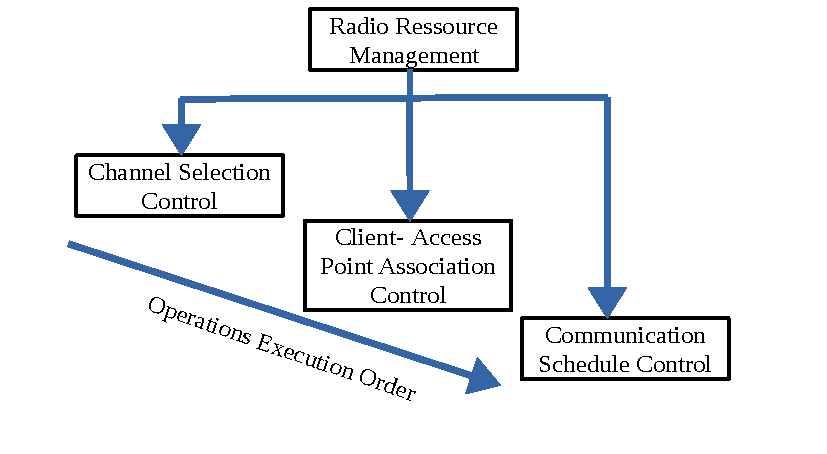
\includegraphics[width=9cm]{Figures/Radio_ressource_management.pdf}
\caption{Radio Resource Management classification}
\label{fig:RRM}
\end{figure}
%==============================================

\section{Survey Methodology (me)}
\label{Taxonomies}
In the following sections, we will highlight the different classes of works that tackle the problem of client associations with the Access Points. In section \ref{centralised_works}, the works will be described according to these classes. In addition, the works will be summarized in tables that contain many key elements. In fact, the majority of the described works in this study will be tagged by their method of performing client association through offline (periodic) control or through online incremental one. As some works suppose that the neighboring Access Points are interfering and so should be controlled in order to avoid transmissions collisions, a box in the table will show if the work takes this into account or not. In practice, as not all the clients consume the offered bandwidth, and as the used application gives an idea about the needed bandwidth, the table contains a box to show the works taking this parameter in the association control or not. Since the presented works propose changes in the association behavior compared to the standard, there will be a change in the software to handle the optimisation. This change could be performed at the Access Point or/ and the client for which a box in our summary table is reserved. The data to be sent is in practice bidirectional but some works interest on one direction (uplink/ downlink) traffic for which the table highlights the information. The majority of presented works in this study formulate the optimisation problem as heuristics, while few ones solve the problem as an exact solution. For that, we try to explicitly show this behavior in our tables. During our study we remarked that some works try to enhance the resulting throughput by allowing the connection with several Access Points at the same time. Even this solution is not largely deployed, but we would like to show the works using it in our tables. Another point that has its major importance in associations is the fact of handling the clients mobility transparently by allowing complete roaming. Our tables show the works that perform the transparent roaming from those don't taking it in consideration through a given box in the table. Lastly, three boxes in our summary table are dedicated to the the evaluation of the proposed work. The first box designs the method of "work evaluation" that could be by simulation, experimentation or analytically. The parameters chosen as performance metrics are also depicted in a box table, in addition to the candidate works that the concerned work chooses for comparison.            

\subsection{Centralised approaches (me)}
In a large WLAN with different cells, the clients could have different link rates according to their associations. These different rates are due to the different modulation used by each client in order to overcome the losses present in the environment. In fact, the clients know different loss and interference in their path. On the other hand, the default DCF function used for each Access Point transmissions leads implicitly to use the rate of the slowest station for individual throughput calculation, as the DCF function ensures packet fairness by giving all the stations the same chance of transmission \cite{03performance_anomaly_DCF}. Such fairness could decrease the aggregated performance as seen by some applications, while other ones consider this type of fairness as the needed one \cite{05performance_time_throughput_fairness}.
The aim of performing a client AP association, different from that of the standard IEEE802.11, is to enhance the network performance. Such performance could be seen differently according to the network organisers to fulfill applications requirements. Indeed, most of the applications need to optimise the network aggregate throughput, while other ones could in addition interest in a certain form of fairness between the different clients. In some cases, the application could also interest to optimise other parameters rather than the throughput, like jitter, energy, and cost. 
In figure \ref{client_AP_association} we depict the motivation behind performing client-AP association optimisation that covers also mobility handling and load balancing purposes. \\

%==============================================
\begin{figure}[t]
\centering
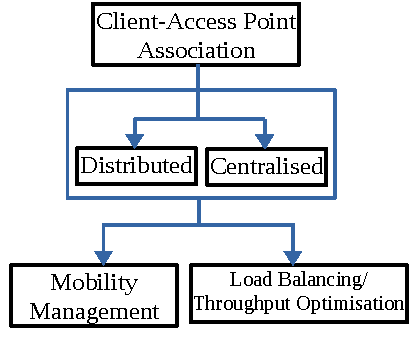
\includegraphics[width=5cm]{Figures/client_AP_association.pdf}
\caption{Client-AP association behaviour}
\label{client_AP_association}
\end{figure}
%==============================================

In order to perform centralised client Access Point association in a network composed of multi cell Access Points, a central controller is necessary to take the decision. This controller could be a chosen AP or a dedicated controller (or management server \cite{08proportional_fairness_multiRate_LAN}). If the network is of a large scale, an hierarchical control could be performed through a multi level control between different sub-level controllers of different sub-networks. The tasks of the controller are not only the client-Access Point association but different control could be performed starting by the channel selection, power control, and communication schedule. With the SDN (software defined networking) approach many other tasks could be envisaged in future according to the applications need like different QOS and reliability requirements, real time constraints, etc...Some coordination between foreign networks could also be performed through the communication between different controllers, even if the association is not envisaged with such networks. The figure \ref{SDN_WLAN} depicts this architecture.\\

The Client-Access Point association optimisation could be formulated as a centralised optimisation problem of a given objective function with the concerned parameters and written as:

$\textbf{max}  \sum\limits F(i,j)$ or  $\textbf{min}  \sum\limits F(i,j)$ \\

These optimisation problems formulations are generally non linear or/ and no convex in their majority, for which the authors propose heuristic algorithms to approximate them. \\

In practice, different forms of fairness could be needed by the application while optimising the throughput through client associations, and the most known ones are Max-min and proportional fairness. Associations using max-min fairness try to enhance the performance of the slowest nodes through maximising the throughput of the minimum one seen in the network. On the other hand, the proportional fairness form tries to share the throughput between the stations in a manner proportional to their rates. In some found works, the aggregate network throughput is maximised without any kind of fairness \cite{15AP_association_MIMO}. In the following sub-sections, we give more details on these fairness forms used for associations, for which some concerned works are presented in section \ref{centralised_works}. While in figure \ref{throughput_and_fairness} a possible classification of client-AP association is shown.

\subsubsection{Proportional fairness based Client Access Point Association} 
As its appellation means, the proportional fairness form of throughput sharing ensures proportionality between the users according to their individual rates or link capacity.
In \cite{97kelly_elastic_rate}, the authors describe in details how logarithmic function used in the objective optimisation function ensures such proportionality. In fact, The presence of the log function in the objective throughput maximisation function encourages a proportionality between the low and high values, as the presence of many low values having low or negative log function values decrease the sum in the objective function which promotes an equilibrium between these values and the high ones in the global objective function. The optimisation problem could be described as the following, while the table \ref{AP association_formulate_table} contains the notations and their meaning used in literature formulations:

%=====================================================
\begin{footnotesize}
\begin{equation}
\left\{
\begin{tabular}{l}
$\textbf{max}  \sum\limits_{j \in U} \log ( \sum\limits_{i \in A} w_{ij} x_{ij} b_{ij}) $ \\         
\\
\textbf{subject to} \\
\\
~~~~~$ \sum\limits_{i \in A} x_{ij} = 1 ~~~~~~~~~ \forall j \in U $ \\ 

\\
~~~~~$ x_{ij} \in \{0,1\} ~~~~~~~~~~~~ \forall i \in A, \forall j \in U $ \\

\\
~~~~~$ b_{ij} = t_{ij} r_{ij}$ ~~~ $\forall i \in A, \forall j \in U $  \\


\end{tabular}
\right.
\end{equation}
\end{footnotesize}

%=======================================================

In addition to this proportionality when maximising the aggregated throughput, the time reserved for transmission could be equal between the clients of the same Access Point, giving birth to the time fairness paradigm. The throughput of the clients in the same Access Point could also be equal, giving birth to the throughput (or access) fairness, too. The following sub-sections give more details on these sub-classes. The figure \ref{throughput_and_fairness} highlights this classification of throughput optimisation with different fairness paradigms.

\paragraph{Access based fairness or throughput based fairness (me)}
The aim of this fairness paradigm is to attribute the same number of channel access to all the clients of the AP. When the rate used by the different clients is the same, this paradigm gives identical results as for the time fairness based one. On the other hand, when the clients have different links rates, the default use of DCF function makes that the clients have the same individual throughput for this fairness type contrary to time based one. The resource considered here to be shared fairly is the packet transmission, and the clients have the same number of channel access, where each access lasts for a different period between them. So the slowest clients in each channel access occupy the medium for a longer time period than the fast clients that occupy the medium for a shorter period for sending the same data \cite{08proportional_fairness_multiRate_LAN}. Considering this behavior explicitly in the association problem formulation will give a better resulting throughput. In the optimisation problem described above, the following constraint should be added in order to take access fairness into account:

$ b_{ij}= \frac{1}{\sum\limits_{k \in U} \frac{x_{ik}}{r_{ik}}} $ ~~~~ $\forall j \in U,  \forall i \in A $  \\


This type of fairness leads to a Max-min bandwidth fairness if used in a single Access Point, as the slowest client has the same throughput as the faster one. For some applications, this kind of fairness is sufficient even if it decreases the overall throughput compared with the case of time based one, as seen in the next section. 

\paragraph{Time based fairness Association(me)}
In the second proportional fairness form, the resource to be considered fairly is the time sharing rather than the throughput at each AP level. For that, the clients of the same Access Point have the same time period in the frame, and each one uses it according to its real rate resulting to individual throughputs proportional to the link capacity rates. This philosophy is used in the intra Access Point policy to share the resources. In fact, multi rate modulation leads to an under utilisation of the network resources with the use of DCF function that gives an equal packet transmission for all the clients which results that the slower clients monopolise the medium for a longer time compared to the fast clients leading to reduced network throughput performance \cite{08proportional_fairness_multiRate_LAN,16rigourous_practical_proportional_fair_AP}. But if the clients are given the same service time period, where each one uses this period to send according to its physical rate capacity, a better proportionality will be fulfilled, and the network throughput will be enhanced. But at the same time, this changes the standard scheduling \cite{16AP_association_optimisation_fairness}, that should be tackled adequately. The optimisation problem formulation should contain the following constraint in order to take time fairness:

$ b_{ij} = \frac{r_{ij}}{\sum\limits_{j' \in U} x_{ij'}}$  $\forall i \in A, \forall j \in U $, where also $ t_{ij} = \frac{1}{\sum\limits_{j' \in U} x_{ij'}}$ \\

In the figure \ref{fig:Time_Access_Fairness}, we depict an example of a network in which three stations have different individual rates while they connect to two Access Points. We show how the aggregate throughput could change according to the different associations (station 2 with AP1 or AP2), and the fairness type (time/access).

\paragraph{Proportional Aggregate throughput in inter AP association (me)}
The third class of works treating proportional fairness tries to ensure proportional fairness between clients, through the logarithmic function, without applying neither time nor access fairness. In fact, in the previous subclasses, the fairness concerns each single AP assignment of clients throughput in addition to the global fairness. In this class, the scheduling should also be tackled in order not to apply the default one using DCF behavior. 

\subsubsection{Max-Min Fairness based Association}
The max-min fairness tries to enhance the performance of the slowest nodes, through maximising the minimum throughput seen in the network. In \cite{06proportional_fairness_3G_networks}, the authors define it as attributing the bandwidth in a manner that any other affectation trying to enhance a user bandwidth leads to decreasing the bandwidth of another client having the equal or less bandwidth. 
There is a close relation between this fairness and that of minimising the load of each Access Point through Min-Max the load of Access Points as proved in \ref{04Fairness_load_balancing_WLAN,07fairness_load_balancing_LAN}


\subsubsection{Other QOS and load balancing based centralised client-AP association works (me)}
Quality of service parameters that are considered by the applications differ according to the application need. In fact, the application could interest to the packet delay or jitter, the overall throughput, etc...which are used for performing load balancing. The optimisation of client association could be performed according to one or some QoS parameters that will be present in the problem formulation or taken into account in the heuristics.  

\subsection{The need of online association/re-association}

In real networks utilisation, the clients could be present at the beginning of the network lifetime, for which an offline optimisation of associations is performed. While in other applications (which is the most realistic) the clients arrive sequentially and could also leave at any moment. Performing the offline optimisation at each change could be expensive and time consuming, in addition to frequent possible disconnection. In this case, it necessitates an online incremental association at each change in the network. This type of association could lead to a suboptimal performance, for which periodic re-association could be a good choice. 

\subsection{Interference between adjacent Access Points} 
In some propositions, the authors suppose that the neighboring Access Points use orthogonal channels being so not in interference and can consequently communicate at the same time, and for other ones the authors suppose denser networks in which the orthogonal channels are not sufficient to be used between the neighboring Access Points and the interference should be taken into account. These information are present at the Access Points level and transmitted into the controller. But in other situations, the interference with other adjacent Access Points could not be seen at the Access Point level, and only the clients that are present in the cross range of the adjacent Access Point could see. For this reason, some works take into account the information brought by the clients, giving birth to Access Point side and client side information based works. Also, in all the works that treat the client-Access Point association, the rate between each pair of client and a candidate Access Point should be taken into account, such information is brought by the AP after the probing messages and responses from the clients, but could be found through the standard messages exchanged \cite{08AP_assignement_algorithms}, too.  \\ 

%==========================================
\begin{figure}[t]
\centering
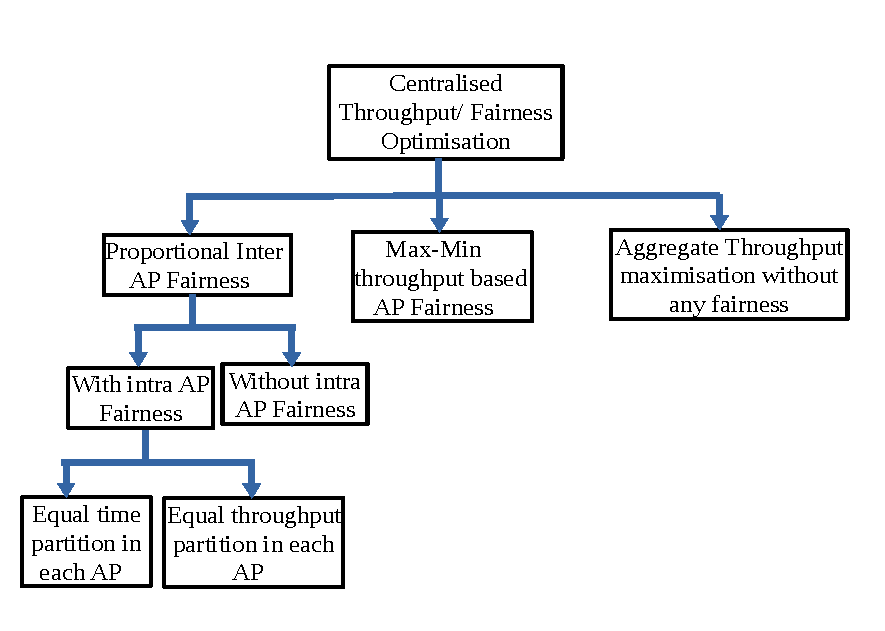
\includegraphics[width=9cm]{Figures/throughput_and_fairness.pdf}
\caption{classification of centralised Clients-AP association fairness}
\label{throughput_and_fairness}
\end{figure}
%================================================

\subsection{distributed (decentralised) approaches}
In this approach, the control of clients associations could be done at the Access Point individually (which could also choose the channel to use and schedule clients communications), while communication with adjacent Access Points is also possible in order to exchange surrounding information. On the other hand, the client could from its side make the association decision by choosing the better Access Point from those in its vicinity. This decision is based on performance parameters that the client gathers from the network or from the beacons sent by the Access Points \cite{17QOS_AP_selection}, such as QBSS load element available in the IEEE 802.11e  \cite{09load_balancing_WLAN}. Generally, the client chooses its better Access Point in a selfish manner that tries to enhance its individual throughput (or other QoS parameter) without thinking about other clients resulted performance nor network wide load balancing, while the Access Point does not perform any decision different from the standard in such case. In \cite{09load_balancing_WLAN}, the authors claim that this selfishness of the client leads implicitly to choose the least loaded Access Point, which is a largely used policy for load balancing. \\
The re-association is also possible with the distributed association strategies. But the problem that should be handled carefully when the association is decided by the client is the continuous Access Point change that may happen and how to cope with. In fact, the presence of a new Access Point in an environment containing many clients already connected with an old Access Point results to the common migration towards this new one, that quickly become loaded, and all the clients come back commonly to the old one and so on. In \cite{09load_balancing_WLAN}, the authors propose to wait for random consecutive periods of verification that the new Access Point still keep less loaded or giving better throughput than the old one before performing the migration.

%=================================================
\begin{center} 
%\begin{footnotesize}
\begin{table}[htbp]
\centering
\begin{tabular}{|c|l|} %\
\hline
Notation 		& Description \\
\hline
$A$				& Set of available Access Points\\
$m$				& Number of concerned Access Points, $|A|=m$ \\
$U$				& Set of all wireless clients \\
$n$				& Number of Concerned wireless clients, $|U|=n$  \\
$C$ 				& Set of available wireless channels\\
$c$		        & Number of total wireless channels, $|C|=c$  \\
$n_i$			& Number of wireless clients in network of AP $i$\\
$P_i$			& Transmission power of AP $i$ \\
$R_i$			& Downlink rate limit of Access Point i\\
$d_{ij}$			& 1 if AP $i$ is in the receiving range of client $j$ \\
$s_{ij}$			& 1 if AP $i$ is in sensing range of user $j$. \\
				& Sometimes used if AP $i$ is in sensing range  of AP $j$\\
$w_{ij}$			& priority of user $j$ on AP $i$ \\			
$r_{ij}^k$ 		& Link rate of client $j$ on AP $i$ using channel $k$\\
$t_{ij}^k$		& Air-time of AP $i$ for user $j$ on channel $k$, \\
				& used for time fairness formulation \\
$b_{ij}^k$		& Bandwidth share of user $j$ on AP $i$ on channel $k$ \\			
$x_{ij}^k$		& associate client $j$ to AP $i$ on channel $k$\\


\hline
\end{tabular}
\caption{\label{AP association_formulate_table} Notations used to formulate the AP association optimisation problem}
\end{table}
%\end{footnotesize}
\end{center}
%======================================


%=========================================================
\begin{figure*}[t!]
\centering
\subfigure[Network topology]{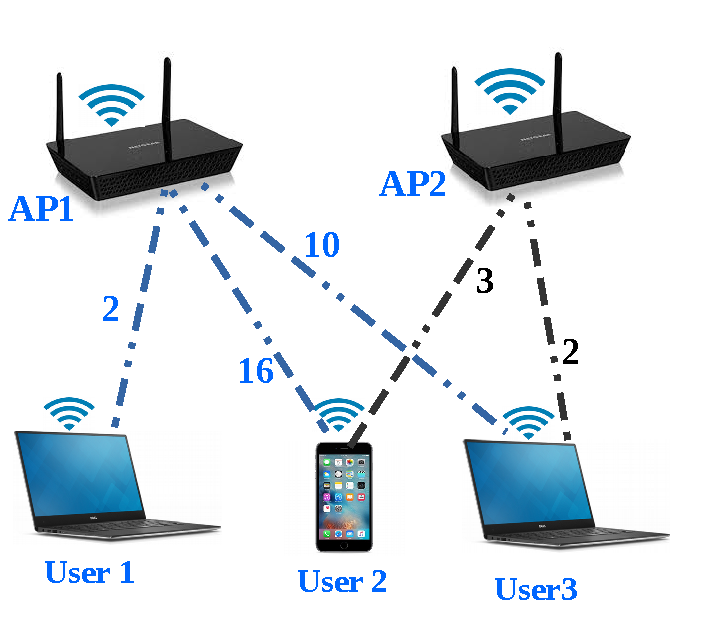
\includegraphics[scale=0.3]{Figures/fairness_2AP.pdf}}
\hfil
\subfigure[Aggregated Throughput]{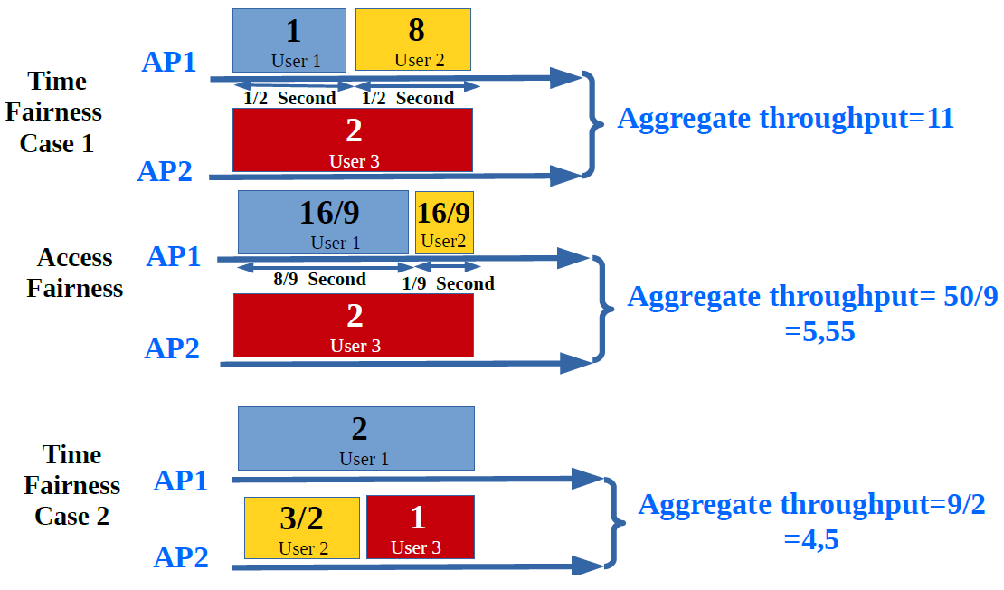
\includegraphics[scale=0.42]{Figures/fair_throu_2AP.pdf}}
\hfil
\subfigure[Aggregated throughput in case 1 Association]{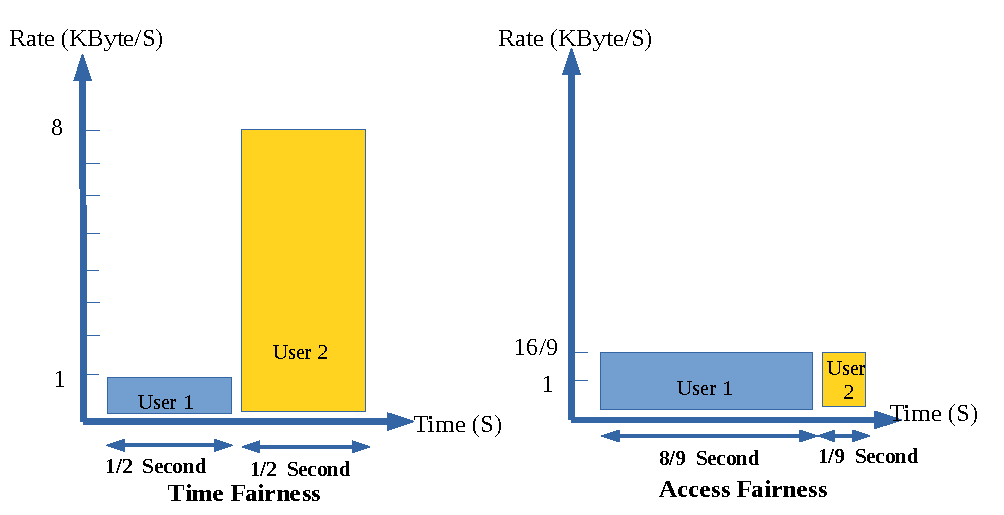
\includegraphics[scale=0.42]{Figures/debit_time_access_2AP.pdf}}
\caption{Example of fairness and the Resulting Aggregated throughput}
\label{fig:Time_Access_Fairness}
\end{figure*}
%===========================================================


\section{Different IEEE802.11 working groups} (me)
\label{802.11 principe}

The standard 802.11 is largely adopted and its utilisation is increasing since its first version in 1997. The standard proposes the use of different frequency bands like 2.4 GHz (norme b/g/n), 5 GHz (norme a/n/ac) and 60 GHz (norme ad). In addition, many working groups related to the standard tackle different aspects related to the network services like QoS (Quality Of service) in 802.11e, the security in 802.11i and vehicular communications in 802.11p. The last revision  of the standard containing all the previous amendments is released by 2016 \cite{16standard_802.11}. In table \ref {IEEE802.11 task groups}, some working groups are depicted treating interesting topics related to WLAN \cite{17CISCO_mobility_guide}, while the next sections describe in more details the amendments that provide interesting information for optimised network resource managements as in 802.11 e/k/r/v \cite{16IEEE802.11k_r_v}.  

%=================================================
\begin{center} 
%\begin{footnotesize}
\begin{table}[htbp]
\centering
%\begin{tabular}{|c|l|} %\
\begin{tabular}{|p{1.cm}|p{7.cm}|}
\hline
IEEE 802.11 Task Groups 		& Activity \\
\hline
$a$				& To develop PHY for 5 GHz UNII band\\
$b$				& To develop higher rate PHY in 2.4 GHz band \\
$c$				& To cover bridge operation with 802.11 MACs (spanning tree) \\
$d$				& To define physical layer requirements for 802.11 operation in \\
				& other regulatory domains (countries)\\
$e$ 				& To enhance 802.11 MAC for QoS\\
$f$		        & To develop recommended practices for Inter Access Point Protocol \\
				& (IAPP) for multi-vendor use\\
$g$				& To develop higher speed PHY extension to 802.11b (54 Mbps) \\
$h$				& To enhance 802.11 MAC and 802.11a PHY-Dynamic Frequency \\
				& selection (DFS), Transmit Power control (TPC)\\
$i$				& To enhance 802.11 MAC security and authentication mechanisms\\
$j$				& To enhance the 802.11 standard and amendments to add channel \\
				& selection for 4.9 GHz and 5 GHz in Japan \\
$k$				& To define RRM enhancements to provide interfaces to higher \\
				& layers for radio and network measurements\\
$m$				& To perform editorial maintenance, corrections, improvements, \\
				& clarifications, and interpretations relevant to documentation \\
				& for 802.11 family specifications \\
$n$				& Focus on high throughput extensions ($>$ 100MB/s at MAC SAP) in \\
				& 2.4GHz and/or 5GHz bands \\
$o$				& To provide Fast Handoffs in Voice over WLAN (goal is around 50ms)\\			
$p$ 				& Focus on vehicular communications protocol aimed at vehicles, \\
				& such as toll collection, vehicle safety services, and commerce \\
				& transactions via cars \\
$r$				& To develop a standard specifying fast BSS transitions \\
				& and fast roaming\\
				
$s$				& To define a MAC and PHY for meshed networks that improves \\
				& coverage with no single point of failure \\			
$t$				& To provide a set of performance metrics, measurement \\
				& methodologies, and test conditions to enable manufacturers, \\
				& test labs, service providers, and users to measure the \\ 
				& performance of 802.11 WLAN devices and networks at the \\
				& component and application level\\
$u$				& To provide functionality and interface between an IEEE 802.11 \\
				& access network (Hotspot) and any external network\\
$v$				& To provide extensions to the 802.11 MAC/PHY to provide network \\
				& management for stations (STAs) \\
$w$				& To provide mechanisms that enable data integrity, data origin \\
				& authenticity, replay protection, and data confidentiality for \\
				& selected IEEE 802.11 management frames including but not \\
				& limited to: action management frames, deauthentication and \\
				& disassociation frames\\

\hline
\end{tabular}
\caption{\label{IEEE802.11 task groups} Different IEEE802.11 task groups activities from \cite{17CISCO_mobility_guide} }
\end{table}
%\end{footnotesize}
\end{center}
%======================================


\subsection{802.11e for QoS enhancing} (me)
The aim of this amendment, which is an enhancement of 802.11b, is to allow different applications to have different quality of service requirements through different priorities for channel access \cite{16standard_802.11}. In fact, Voice on IP application should have higher priority than a TCP based one in order to ensure acceptable execution. The HCF (Hybrid Coordination Function) proposed in this amendment allows to access the channel in contention-based, and non-contention based modes. In EDCF (Enhanced Distributed Coordination Function), which allows the access in contention based mode, and is considered as an enhancement of DCF, the prioritised channel access is performed by defining AC (Access Categories). Indeed, each station possesses 4 categories, and each one could have different priorities of applications at the same time. In this manner, each category could be considered as a virtual station, having its own queue and performing contention operation differently than the other categories. In the section \ref{DCF and its problems} describing the DCF functioning, a highlight of EDCF functioning is also given for contention window choice.    


\subsection{802.11k, radio resource measurement} (me)
The aim of this amendment is to give information to the stations about their surrounding radio environment, by allowing them gathering and sharing information about their radio links performance, in a manner independent of vendor devices (contrary to RSSi values \cite{16IEEE802.11k_r_v}). For that, this amendment allows the station to gather these values locally, to request them from other stations (by requesting them to perform measurement), or also to respond to stations requesting this information. These radio environment measurements will be available for use by other applications and protocol layers \cite{16standard_802.11} in order to enhance the station resource performance and utilisation. The gathered information are used by applications to enhance reliability (for example VoIP and Video on IP) and to decrease interference in harsh environments (for examples airplanes, factories). The gathered information could also be used for mobility management when the application is resource hungry, by knowing the channel state of the neighboring Access Points, for example. The management frames are changed in order to allow the radio information to be contained and to tag the capability of stations to support the amendment. Indeed, neighboring radio information is the first step towards any smart resource management \cite{16standard_802.11}.    

\subsection{802.11r, fast basic service set transition} (me)
The aim of this amendment is to allow stations to roam in the same ESS (Extended Service Set) between two BSS (Basic Service Set) cells with reduced transition time in order to reduce the data disconnection period, also named fast transition. In practice, in order to roam thorough a new neighbor Access Point, the station should first discover the neighboring Access Point and choose between them the one with which the authentication step will be executed. As these steps consume time, it will cause long disconnection. The 802.11r consists to reduce this period while keeping the same security level as the 802.11i and the same QoS performance as 802.11e \cite{16IEEE802.11k_r_v}. This is performed through negotiating the parameters with the new Access Point (belonging to the same ESS, also named mobility domain) before disconnecting with the current one, which is also named FT (Fast Transition). The 802.11r amendment allows stations to make a 4 steps FT handshake with the Access Points of the same mobility domain from the beginning (through the authentication steps) in order to anticipate the roaming in future. The station should negotiate the authentication according to the need or not of QoS resources, performing so FT with or without resource request. In fact, in the case that the station should apply 802.11e functions, the resources should be reserved on the new Access Point, through two different mechanisms. Namely, the station could negotiate the resources directly with the new Access Point or through the DS by the current Access Point \cite{16IEEE802.11k_r_v}.   

\subsection{802.11v, Wireless network management (WMN)} (me)
In this amendment \cite{16IEEE802.11k_r_v}, network information state are exchanged between stations in order to be aware of the surrounding and for that the resource management or decisions performed by the stations will be optimised. In fact, the stations could be aware about the topology and network information through the exchanged information. The interference presence and its values also could be exchanged between the stations in order to modify their RF choices accordingly \cite{16standard_802.11}. This amendment allows also the exchange of location information as it is useful for many ressource management or application decisions. The stations could also use the sleep mode in which they don't receive the frames from the Access Point during a given long period in order to concerve energy or also to decrease interference. In addition, the amendment handles the group addressed frame delivery and supports performing multiple BSSID capability inside the same infrastructure. The 802.11v amendment could be seen as an extension or complement to the 802.11k that performs radio measurements but with more services and information \cite{16IEEE802.11k_r_v}. 

\section{DCF work Principle (me)}
\label{DCF and its problems}
In the IEEE802.11b standard, there are two access or scheduling mechanisms, namely the Point Coordination Function (PCF) and the Distributed Coordination Function (DCF). In addition, a combination of the two methods could be applied. In PCF, the access to the medium is ensured in a non contended manner through the arbitration of the Access Point as a coordinator. In this manner, the access to the medium is performed in a predefined time shared base, where each station knows its time bounded waiting. This method is well suited for real time applications. Also, priorities of applications could be used in order to promote some users than others, but PCF method is not implemented in 802.11b \cite{03performance_anomaly_DCF}. On the other hand, DCF allows a contention based access to the medium through using CSMA/CA based communications. In this manner, a best effort based service is provided by DCF \cite{03performance_anomaly_DCF}. The communication principle of CSMA/CA is that each station desiring to send a packet should sense the channel before the transmission. If the channel is free, the station waits for DIFS (Distributed Inter Frame Space) period to ensure that the channel is still empty. If this is the case it can send the packet. The receiver from its side sends an ACK packet. If this ACK is not received by the station, it assumes a collision happening and retransmits the packet again after a DIFS period of channel freeness to which it adds a random time period. \\
In practice, many stations would like to transmit at the same time, that leads to finding the channel busy by the candidates at the moment of sensing the channel. In case of channel busyness, the station waits until the channel becomes idle for the DIFS period after which it should execute a collision avoidance mechanism, also named backoff operation, consisting to wait for the backoff period. In fact, it has to wait for a random period between 0 and CW, multiplied by the slot period (slot period =20 μs in IEEE802.11b). Each time the waiting period is decremented by one slot, the channel is again sensed in order to continue the decrementing on condition it is idle. In case the channel is again busy, the decrementing operation is frozen until the channel becomes idle, and DIFS period is again waited. After the backoff value becomes zero, the station could transmit. The CW (contention window) varies between 31 (in 802.11b \cite{15time_fairness_MAC}, and 15 in 802.11 using OFDM like in g/n \cite{16standard_802.11})and a maximum value of 1023. Indeed, the CW starts by 31 and is doubled each time the communication fails until reaching the maximum value after which it keeps on that value. The communication fails and a collision is supposed happening by the non reception of ACK. When the transmission successes, the CW value is coming back to the smallest one, namely 31 in IEEE 802.11b \cite{15time_fairness_MAC}, and 15 for the 802.11 standard using OFDM (like 802.11 g/n) \cite{16standard_802.11}. In practice, the station that chosen the smallest period between the stations starts the transmission at first. When the number of contending stations increase, the performance of such mechanism decreases significantly because of the back off mechanism.\\

With EDCF proposed mechanism in 802.11e standard \cite{11user_centric_management_WLAN}, different stations having different priorities translate to different contention windows selection intervals. In fact stations, with high priorities choose their CW values in an interval having the smallest CW values (in their minimal and maximal values) compared to stations having less priorities. In addition, AIFS (arbitrary inter-frame space) period is used for sensing channel rather than DIFS, and its period is with relation to the priority where the higher priority stations use the smallest AIFS values compared to the less priority ones \cite{05load_balancing_802.11e}. 

In real environment, link qualities are different because of obstacles and interference which cause that the signal received power by the stations is also different. For having good reception ratio in such situations, different MCS (Modulation and Coding Schemes) should be so used. Lower indexes MCS take in consideration channel errors better than higher indexes schemes but lead also to lower links rates \cite{16rigourous_practical_proportional_fair_AP,08AP_assignement_algorithms}, which motivates the use of multirate links in real scenarios. The authors in \cite{14AP_association_multirate_WLAN} show how the link bit rate of a user $j$ associated to an Access Point $AP_i$ is calculated according to the SINR (Signal-to-Interference-plus-Noise Ratio). The result of such bit rate is depicted in table \ref{SINR_rate}, while the following equation shows how the SINR ($\gamma_{ij}$) is calculated:\\
$\gamma_{ij}= \frac{g_{ij}. P_i}{\sum\limits_{K \in A_j\cap k \neq i} g_{kj} P_k + N_0}$ \\
$g_{ij}$ represents the channel gain attributed to client $j$ by the $AP_i$ , $P_i$ is the transmit power of the $AP_i$, $N_0$ is the additive Gaussian white noise, while the set $A_j$ represents the Access Points that interfere with user $j$ transmission.

In practice, even a station has multiple packets to send using DCF mechanism, it has to perform the probing operation after each transmission in order to ensure bandwidth fairness between all the stations through equal transmission opportunities \cite{16rigourous_practical_proportional_fair_AP}. This phenomena leads that stations having slowest rates get the medium for longer periods than the other stations at each transmission using the actual rate, and leading to an equal long time throughput for all the stations, which is relative to that of the slowest station rate degrading so the overall throughput \cite{03performance_anomaly_DCF,07optimal_association_MSWIM}. But in a network containing clients with very high link rate, as that of 802.11 ac/n, this behaviour dramatically curb their capacities \cite{16rigourous_practical_proportional_fair_AP}. This beahviour is known as DCF anomaly and pushes to traffic control research works as we will describe in the following sections.     

\begin{center} 
\begin{footnotesize}
\begin{table*}[t]
\centering
\begin{tabular}{|c|l|l|l|l|l|l|l|l| } %\
\hline
$\gamma_{ij}$(db) & 6-7.8 & 7.8-9 & 9-10.8 & 10.8-17 & 17-18.8 & 18.8-24 & 24-24.6 & 24.6- \\
\hline
$r_{ij}$ (Mbps) & 6 & 9 & 12 & 18 & 24 & 36 & 48 & 54  \\\hline


\hline
\end{tabular}
\label{SINR_rate}
\caption{The relation between SINR and effective rate}
\end{table*}
\end{footnotesize}
\end{center}

\section{Standard association of clients to AP in 802.11} (me) 
For using the 802.11 WLAN network to communicate with another station by sending or receiving traffic, each station should be first connected to a given Access Point. This connection, named association is performed thorough four steps as depicted in Figure \ref{fig:Association_client_Access Point}. Before associating to a given Access Point of the network, named also \textit{BSS (Basic Service Set)}, this one should be discovered by the station in a first step and this operation is called \textit{scanning} and could be performed in an \textit{active} or \textit{passive} manner. The \textit{active scanning} consists that the station sends a \textit{Probe request} frame on each channel. The Access Points of its vicinity present on each channel respond by a \textit{Probe response} frame. On the other hand, in a \textit{Passive scanning}, it's the Access Points that broadcast periodically \textit{Beacon} frames containing the same information as the \textit{Probe response} frame \cite{08Design_high_wifi_entreprise} and the station listens to these \textit{Beacons}. The second step consists to choose one Access Point from the collected ones. The standard operation of 802.11 bases this selection on the strongest RSSI (Received Signal Strength Indication) of the \textit{beacon/ Probe Response} frame. Before associating to the chosen Access Point, a third step consists to an \textit{authentication} by the Access Point, if it performs such mechanism. As a fourth step, the station sends an \textit{association request} frame to the Access Point for which this last answers by an \textit{Association Response} frame. This frame contains the decision taken by the Access Point that could be positive or negative, according to the \textit{successful} or \textit{failure} status indicator \cite{11contention_traffic_load_aware_association,07optimal_association_MSWIM}. The standard 802.11 allows the Access Points to respond or broadcast a null SSID, named also \textit{hidden SSID} to stations that should send in their request the correct SSID to get the association. In the case of not sending this value, the Access Point does not respond \cite{08Design_high_wifi_entreprise}.

%==============================================
\begin{figure}[t]
\centering
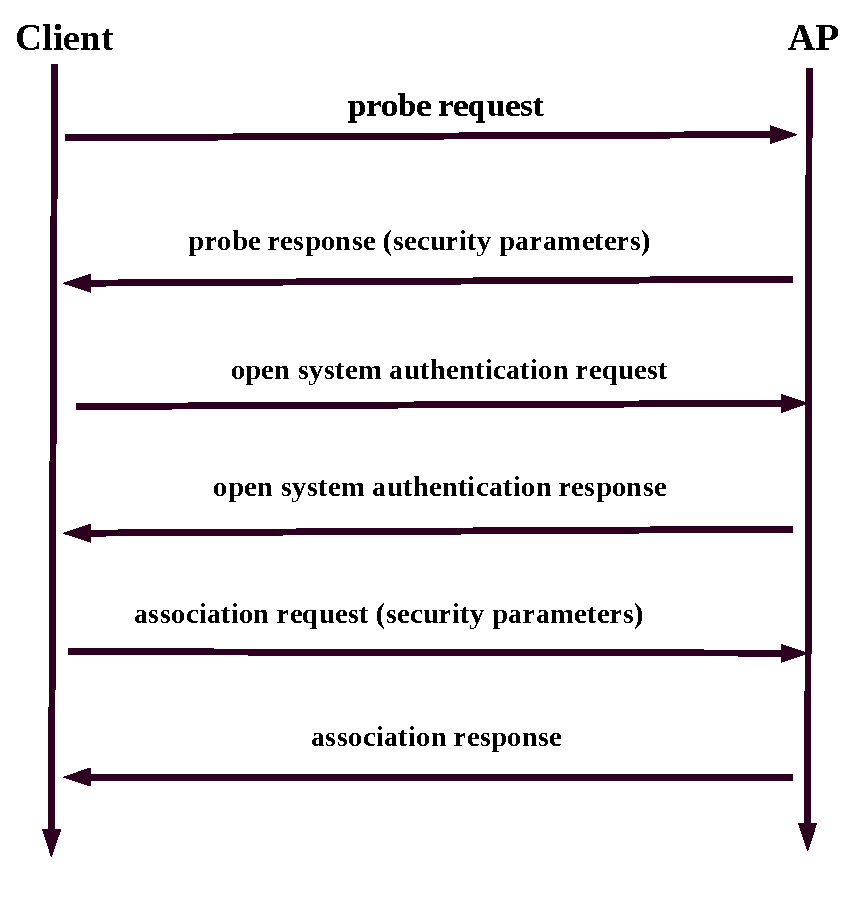
\includegraphics[width=5cm]{Figures/Association_standard.pdf}
\caption{Messages exchange for Client-AP Association using 802.11}
\label{fig:Association_client_Access Point}
\end{figure}
%==============================================

\section{Performance Evaluation Metrics for Access Point Association} (me)
\label{evaluation parameters}
In literature, the proposed works for client Access Point association are evaluated through simulations like in \cite{10approximate_optimisation_proportional,14AP_association_multirate_WLAN,11proportional_fairness_power_control,15Demand_aware_load_balance_WLAN,16throughput_optimisation_association_bandwidth,14optimalAP_INFOCOM,12Network_cooperation_AP_association} or through experimentation testbeds like that in \cite{10Dyson,08Design_high_wifi_entreprise,17building_SDN_entreprise_virtual_AP,16VALI_SDN,15OpenSDWN_home_entreprise_WIFI,14Odin:Programmatic_Orchestration_WiFi,06practical_queue_based_AP_association,15fuzzy_load_balancing_802.11,14load_handoff_SDN}. For that, many performance evaluation metrics were used to proof the adequacy and performance superiority of the works compared to the standard ones or to previous proposed methods. The most used performance evaluation parameters in literature works are described in the following:  

\subsection{throughput}
It is the first parameter to be tackled and optimised by any proposition \cite{10approximate_optimisation_proportional,14AP_association_multirate_WLAN,15Demand_aware_load_balance_WLAN,16throughput_optimisation_association_bandwidth,14optimalAP_INFOCOM,12Network_cooperation_AP_association,11proportional_fairness_power_control}. In fact, the throughput is the number of packets correctly received by the Access Point during a period of time, in the case of uplink traffic. If these packets concern all the stations, the throughput is named aggregated throughput. If the measure concerns each station individually, it is named individual throughput. Some times the average of individual throughputs is used, too. With downlink traffic, it is the number of packets received at the level of each station that gives the throughput values, and the previous types of throughput could be also evaluated. 

Theoretically, according to the physical rate of the link between a station $U_i$ and the Access Point $AP_j$, the individual throughput has a relation with the time portion given to the station, taking into account that other stations $U_k$ should be connected to the same Access Point $AP_j$. For example, in the case of no losses and supposing the stations have the same time portion with the Access Point, each station will have a theoretical throughput of $Through_{ij}=\frac{r_{ij}}{Number \ of \ users \ of \ AP_j}$. On the other hand, if the stations of the same Access Point should have the same throughput, its value is supposed to be $Throu_{ji}= \frac{1}{\sum\limits_{u \in U_i} \frac{1}{r_{ui}}}$

In \cite{07optimal_association_MSWIM}, the authors define the average station throughput as: 
$Throu_{ji}= \frac{L_j}{\sum\limits_{u \in U_i} t_{ui}}$. Where $L_j$ is the data length (in bits), and $t_{ij}$ is the needed time by the station $j$ to send this data over $AP_i$.

In practice, the throughput value depends on the number of stations connected to the Access Point and the neighboring interfering Access Points \cite{16AP_association_optimisation_fairness}.   

\subsection{Average Blocking Probability} This parameter quantifies the refusal probability of new arriving users, as they decrease the average throughput (or satisfaction) of the already connected ones by a given percentage. Each time a new user is accepted, the probability value is changed \cite{17QOS_AP_selection}.   

\subsection{Average Satisfaction} It quantifies the percentage of users having given their bandwidth demands or more. This value changes according to the used applications and the number of users, too \cite{17QOS_AP_selection}.   

\subsection{Average Data Bit Rate} It has the same meaning of the average individual throughput, as it quantifies the effective data bit rate per second given by the Access Point to its associated clients \cite{17QOS_AP_selection}. 

\subsection{Jain's fairness index} 
The aim of this index is to measure the degree of fairness of a given parameter between the candidates present in the Jain equation. For Access Point Association strategies, the parameter that should be given fairly, according to a certain level, is the bandwidth. As the stations are given the bandwidth equally, as the value of Jain's fairness index is close to $1$, and inversely, as the stations are given dissimilar bandwidth values the value of this index approaches to $0$ \cite{14AP_association_multirate_WLAN}.  
Given the number of users is $M$, the equation of bandwidth Jain's fairness index is given by:
$j=\frac{\left(\sum\limits_{i=1}^M b_{ij}\right)^2}{M \sum\limits_{i=1}^M {b_i}^2} $

In \cite{15Demand_aware_load_balance_WLAN,16throughput_optimisation_association_bandwidth}, the authors measure both time and bandwidth fairness using the Jain's index in order to show the adequacy of their scheme.

\subsection{AP load}
This metric reflects the degree of non ability of the Access Point to answer the clients needs in terms of bandwidth \cite{04Fairness_load_balancing_WLAN}. In literature, many measurements were used in order to estimate the Access Points load like the number of associated users, the measured channel ratio and the delay seen by the clients to receive the beacons messages \cite{14online_AP_association_80211n}. In \cite{04Fairness_load_balancing_WLAN,08AP_assignement_algorithms}, the authors claim that the load is inversely proportional to the average bandwidth and is expressed by the necessary time to complete the traffic transmission of the associated users. In \cite{09load_balancing_WLAN}, the authors propose to use thresholds values to consider Access Point as under loaded or overloaded. Also, the same authors introduce the relative load, where the concerned Access Point load is compared with the average value by a given amount.  

\subsection{balance index} 
This index is calculated with the same manner of Jain's fairness index, but with replacing the ressource value seen previously, which could be the bandwidth or the time period, by the value of the load $L_i$ applied or characterizing the Access Point $AP_i$ \cite{09load_balancing_WLAN}. It quantifies if the $n$ Access Points are loaded fairly or not. The same reasoning of Jain's fairness index is also applied on the obtained values, and so values close to 1 mean that the Access Points are loaded fairly, while values close to 0 mean that there is an unbalance on the Access Points load. The balance index $β$ is defined as: $β =\frac{(\sum L_i)^2} {n \sum{L_i}^2}$

\subsection{per-packet delay} In some works, the association takes into account real time traffic of users where deadline constraints are prioritised than strict reliability. Therefore, this metric evaluates the delay cumulated in transmitting queues at the senders in addition of that seen at the MAC level because of the collisions and the backoff. The aim of this metric is to show the adequacy or not of the proposed method to answer the realtime, like voice, traffic \cite{06client_channel_WLAN}. 


\subsection{competitive ratio} 
The aim of this metric is to calculate the ratio between the observed value and the optimal one. It can be used to evaluate throughput, Access Point load, ...In some works (for example\cite{13smartAssoc}), this metric is used to express the load balance between the Access Point. For that, large values are not a good sign, while the value 1 is good to say that the ratio between the optimal load value and the seen one are not far from each other. 

\section{Centralised approaches (me)}
\label{centralised_works}
In order to perform centralised client Access Point association in a network composed of multi cell Access points, a central controller is necessary to take the decision. This controller could be a chosen AP or a dedicated controller (or management server \cite{08proportional_fairness_multiRate_LAN}). If the network is of a large scale, an hierarchical control could be performed through a multi level control between different sub-level controllers of different sub-networks. The tasks of the controller are not only the client-Access Point association but different control could be performed starting by the channel selection, power control, and communication schedule. With the SDN (software defined networking) approach many other tasks could be envisaged in future according to the applications need like different QOS and reliability requirements, real time constraints, etc...Some coordination between foreign networks could also be performed through the communication between different controllers, even if the association is not envisaged with such networks. The figure \ref{SDN_WLAN} depicts this architecture.\\
 
%==============================================
\begin{figure*}[t]
\centering
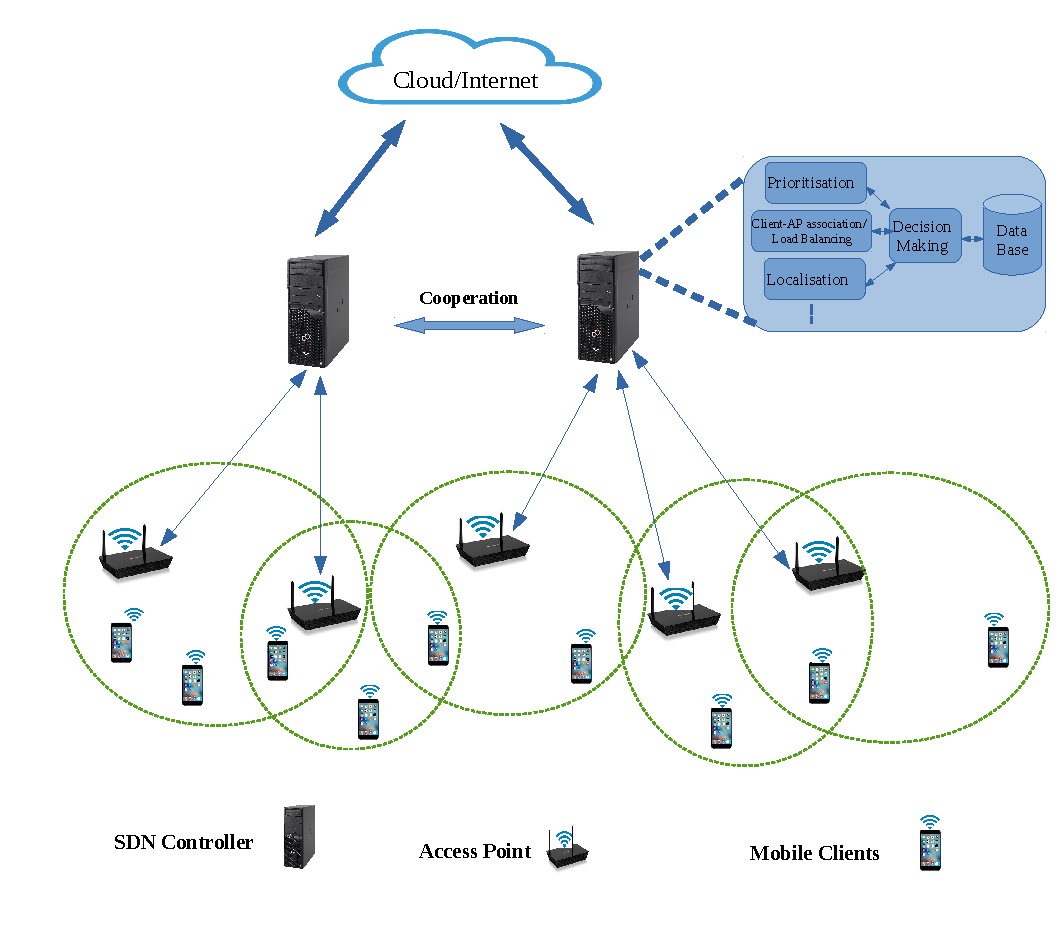
\includegraphics[width=12cm]{Figures/SDN_Controller_WLAN.pdf}
\caption{A possible architecture of SDN based centralised Controller WLAN}
\label{SDN_WLAN}
\end{figure*}
%============================================== 
 
The aim of performing a centralised client AP association, different from that of the standard IEEE802.11, is to enhance the network performance. Such performance could be seen differently according to the network organisers to fulfill applications requirements. Indeed, some applications need to optimise the network aggregate throughput, while other ones could interest in a certain form of fairness between the different clients. In some cases, the application could interest to optimise other parameters rather than the throughput, like jitter, energy, and cost. \\
In a large WLAN with different cells, the clients could have different rates according to their associations. These different rates are due to the different modulation used by each client in order to overcome the losses present in the environment. In fact, the clients know different loss and interference in their path. The default DCF function used in such cases leads to use the rate of the slower station, as the DCF function ensures packet fairness by giving all the stations the same chance of transmission \cite{03performance_anomaly_DCF}. Such fairness could decrease the performance as seen by some applications, while other ones consider this type of fairness as the needed one \cite{05performance_time_throughput_fairness}. In practice, different forms of fairness could be needed. The max-min fairness tries to enhance the performance of the slowest nodes, through maximising the throughput of the minimum one seen in the network. The other form of fairness tries to share the throughput between the stations in a manner proportional to their rates. The first type of fairness (max-min) could be ensured at the AP level leading to access fairness in which the throughput of all the clients of the same Access Point are equal. This is ensured by giving them an access time according to their physical rate capacity. While in the second proportional fairness form at each AP level, the time fairness is used, where the clients of the same Access Point have the same time period in the frame, and each one uses it according to its real rate resulting to individual throughputs proportional to the link capacity rates. This philosophy is used in the intra Access Point policy to share the resources. In addition to this view, an inter APs proportionality could be used and optimised between the clients to choose where they will be associated by introducing the logarithmic function in the objective function that will be optimised by the central controller. This objective function is described in detail in \cite{97kelly_elastic_rate}. The logarithmic function could be used in the global objective function without access or time fairness specification in the same AP, which leads to an implicit access fairness (as the DCF function will do it by default), unless the DCF function is deactivated leading to a proportional fairness between the clients of all the Access Points. In fact, The presence of the log function in the objective throughput maximisation function encourages a proportionality between the low and high values, as the presence of many low values having low or negative log function decrease the sum in the objective function which promotes an equilibrium between these values and the high ones in the global objective function. In some found works, the aggregate network throughput is maximised without any kind of fairness \cite{15AP_association_MIMO}. In Fig.\ref{throughput_and_fairness} a classification of throughput optimisation with different fairness paradigms is highlighted.\\
In real networks utilisation, the clients could be present at the beginning of the network lifetime, for which an offline optimisation of associations is performed. While in other applications (which is the most realistic) the clients arrive sequentially, which necessitates an online incremental association. This second type of association could lead to a suboptimal performance, for which periodic re-association could be a good choice. For the offline client-Access Point association, many works formulate the association as a programming problems which are non linear and no convex in their majority, for which the authors propose heuristic algorithms. \\

In some propositions, the authors suppose that the neighboring Access Points use orthogonal channels being so not in interference and can consequently communicate at the same time, and for other ones the authors suppose denser networks in which the orthogonal channels are not sufficient to be used between the neighboring Access Points and the interference should be taken into account. These information are present at the Access Points level and transmitted into the controller. But in other situations, the interference with another adjacent Access Point could not be seen at the Access Point level, and only the clients that are present in the cross range of the adjacent Access Point could see. For this reason, some works take into account the information brought by the clients, giving birth to Access Point side and client side information based works. Also, in all the works that treat the client-Access Point association, the rate between each pair of client and a candidate Access Point should be taken into account, such information is brought by the AP after the probing messages and responses from the clients, but could be found through the standard messages exchanged \cite{08AP_assignement_algorithms}. In the following section, some protocols using these approaches are described. \\  


\subsection{Proportional fairness based Client Access Point Association} 
\subsubsection{Time based fairness Association(me)}
As explained in the previous section, in a real environment, the stations could have different loss rates due to different interference levels. This leads to use different MCS (modulation and coding schemes) to overcome these losses. In fact, with different modulation, the messages are coded with different levels or redundancy that lead to a slower rate if the redundancy level is high. But this multi rate modulation leads to an under utilisation of the network resources with the use of DCF function. Indeed, DCF gives an equal packet transmission for all the clients in such environment which results that the slower clients monopolise the medium for a longer time compared to the fast clients leading to reduced network throughput performance \cite{08proportional_fairness_multiRate_LAN,16rigourous_practical_proportional_fair_AP}. But if the clients are given the same service time period, where each one uses this period to send according to its physical rate capacity, a better proportionality will be fulfilled, and the network throughput will be enhanced. But at the same time, this changes the standard scheduling \cite{16AP_association_optimisation_fairness}. In this section, the presented works perform their client-AP association, with a time fairness purpose which leads to a proportional fairness, too. We summarise the works of this section in table \ref{Tab:centralised_time_fairness} 


\paragraph{AP Association for Proportional Fairness in Multirate WLANs} (me)
\cite{10approximate_optimisation_proportional,14AP_association_multirate_WLAN}\\
In order to maximise the whole network throughput (total users bandwidth utilities) in a proportional fair manner, authors formulate the problem of client-AP association as a non linear program. A centralised algorithm for the approximation of the non linear program optimisation, dubbed NLAO-PF, is proposed and consists in four steps. The first step is the resolution of the relaxed integral association of users to AP by allowing the associations to all the AP. At the same time, a function for compensating the gap of the integrality association is added in the same optimisation problem. The result of this step is the time affectation of each user to many APs, and this step is executed in a polynomial time. The second step of the algorithm consists to resolve a convex problem in which the association to APs is a variable and the time associated from the first problem is taken as an input. The result of this step will affect each client to a given number of APs, and not to all the APs (as done in the first step). The third step of the algorithm consists to round the association of each user to only one AP. The last step of the algorithm consists simply to assign the time fraction in a proportional fair between the users of the same AP by dividing the time equally. The authors proved that the algorithm offers at least half of the optimal solution. The execution of NLAO-PF algorithm is done periodically as it is expensive and could not be executed at each user arriving or leaving. In order to overcome the arriving or departure, an online distributed heuristic, dubbed BPF (Best Performance First), is performed to allow the association of the new arriving users to the best AP, waiting for the next centralised periodic association calculation. Also, for the leaving users, their resources are shared between the clients of the same AP. The metric consists to calculate the difference of the AP utility that the new user will add to the associated AP, and chooses the one that offer the maximum AP utility gain. Authors claim that they take users mobility into account by performing de-associations/ re-associations operations based on AP load and SINR, while trying to minimise the number of these operations to ensure communication stability. But for the user this is not transparent. So, we consider that this is not a full mobility handling in a transparent manner. We have considered in our classification of the protocol only the centralised part issued from the centralised optimisation heuristic, while in reality the protocol uses also the distributed part to choose for the new user association. \\

\paragraph{Achieving proportional fairness via AP power control in multi-rate WLANs} (me) 
\cite{11proportional_fairness_power_control}\\

The authors consider the proportional fairness paradigm for throughput maximisation in dense multi rate WLANs, by performing power control of APs transmission. The resulting power control will lead to client re-association, according to the standard client association of IEEE 802.11 with the AP having the strongest signal. The problem is formulated as a non linear optimisation problem for simultaneous power control and client-AP association that leads to a tradeoff between fairness and network throughput. A centralised heuristic is proposed in order to resolve the NP-hard problem. The authors establish a relation between the network and AP utilities, and their algorithm, PCAP (Power Control for AP performance), has as an aim to increase the average network utility and decrease the variance of AP utility. The authors define the AP utility as the weighted bandwidth product of all users associated with the AP. They demonstrate that maximising the AP utility, while minimising the variance between the AP utilities lead to a maximum for the network utility. For that, the PCAP algorithm, that performs bandwidth allocation to users in a proportional fair manner, is composed of two sub algorithms, namely MAP that Maximises the Average Performance of AP utility, and MPV that Minimises the Variance of the AP utility. The functioning of the two sub algorithms (adjusting AP utility) is performed according to power control of AP transmissions. The transmission power change leads to client-AP re association according to the standard. The algorithm starts by using the maximum power for the APs, and each client connects to the AP that offers the strongest signal connection. The decreasing of power in the first algorithm will lead to reducing the interference between APs, resulting to enhancement of the APs utility. The algorithm works in an iterative manner. In the second algorithm, power increase or decrease is performed in order to decrease the variance. The authors show through the simulation results that the power control levels will not present a meaning amelioration with the number of levels over a certain number. The authors take into account the interfering AP in the calculation of the SINR, but they don't take it in the proportional fairness sharing of time associations.\\

\paragraph{Network cooperation for client-AP association optimization \cite{12Network_cooperation_AP_association}} (me)\\ 
In this paper, authors tackle the problem of foreign networks interference and their consequences on the concerned centralised controller decision. They show how this can affect the performance of the concerned network, and propose to formulate the client-AP association as an optimisation proportional fairness problem in a cooperative manner (taking into account these interferences).   
The difference with the work in \cite{14optimalAP_INFOCOM} is that, in the current work, interference is supposed and taken into account between foreign networks, and intra network Access Points are supposed using orthogonal channels to avoid interference. But as being in a foreign network, association of clients could not be done with those networks. While in \cite{14optimalAP_INFOCOM}, the interference between intra network Access Points is supposed for a non sufficient number of orthogonal channels, and possible associations are envisaged. For that, in \cite{14optimalAP_INFOCOM}, the central control of the whole interfering Access Points will bring more refined performance than that done independently by each controller.  

The optimisation problem is formulated as a non linear problem to assign the clients to the appropriate Access Point in a proportional fair manner. The cooperation between these networks consists to share the channel state information (for each AP) in order to allow knowing interference happening.     
The interference is caused differently according to the number of AP in the surroundings with the used power emission and different rate sending. For that, the authors propose that the neighbouring networks should exchange information about the operating channels (for each AP) and their location, periodically, in order to be taken into account in the problem formulation. For overcoming the problem of hidden terminals, that manifests by the received strong signals at a client from an AP that is not in the carrier sense vicinity of the associated AP, the authors propose to further lowering the resulting channel access time, rather than introducing the participation of the clients in such information gathering. The authors propose to use the same algorithm of \cite{08proportional_fairness_multiRate_LAN} in order to solve the non linear cooperative problem.

\paragraph{Optimal Collaborative Access Point Association in Wireless Networks \cite{14optimalAP_INFOCOM}} (me)

The authors tackle the problem of bandwidth sharing in the case where different home connections' belong to the same Internet provider. Each client has its own local Access Point that serves the local devices in the home, in addition to the foreign devices belonging to clients of the same provider far away from their homes (ex: in a city where the buildings connections are present across the different roads, allowing a client to associate to different Access Points in its vicinity). The use of a centralised solution, in which the bandwidth of local Access Points serves the non local clients in addition to the local ones, ensures a higher throughput by an optimised clients associations. The share of the whole network bandwidth is done in a proportional fair manner by giving the same sharing time to the clients having the same priority with differentiation of local and foreign ones. The resulting throughput for each client depends on its link capacity with the associated Access Point. The centralised client associations takes into account the interference between the different Access Points that share the same orthogonal channel, due to the lack of channels in dense WLAN networks. Each client starts by connecting to its local Access Point, or by the one having the strongest signal, waiting for the optimisation process running at the central level. The clients that don't have the software installed will perform a normal not optimised connection.\\ 
The first solution is formulated as a non linear optimisation problem for which the authors propose the use of relaxation, which means that each client could associate to different Access Points, and the problem become a discretized linear program. As a second step, they propose using rounding methods to choose only one Access Point. In this solution the time is shared equally between the clients of the same Access Point, for which we classify the solution as time-based fairness. \\ 
In a second variant of their solution, the authors motivate the use of virtualization paradigm, that allows a client to associate with different Access Points at the same time using the the same radio interface. The resulted optimisation problem is convex and the authors solve it using CVX. For this solution, proportional fairness only is used through adding the log function into the utility function to optimise, without the time or access fairness paradigm. The authors perform a rounding step to ignore some solutions less than a given rate. \\
But the authors don't give details on the periodicity of running the optimised association, because it is not practical to run at each client joining. The hidden terminal problem is not also treated in the multiple association part, even the interference problem is taken into account in the single assignment part. The clustering approach based on localisation that is proposed by the authors to limit the number of variables in the optimisation problem is an  advantage, but could not be always used, specially if there is no disconnections limits in the whole network. \\ 

\paragraph{Throughput Optimization via Association Control in Wireless LANs \cite{15Demand_aware_load_balance_WLAN,16throughput_optimisation_association_bandwidth}} (me) 
The motivation of this work is that authors take into account the different users demand, for clients-AP association in a multi rate scenarios, contrary to the previous studies in this section which suppose that users consume all the given bandwidth. Even the work in \cite{07optimal_association_MSWIM} tackles the user activity notion, but the formulation was not so clear and rigorous. The authors justify the diversity of clients bandwidth demand by the difference in bandwidth between the different network applications. So the charge of each AP will not be resulted from only the number of associated clients, but also according to their individual charge. The authors formulate an optimisation problem where the users demands are added as constraints for enhancing the total throughput in a proportional fair manner, through the use of the bandwidth utility. The resulting problem is a non linear mixed integer one for which the authors propose an algorithm, MABU (Maximum Aggregated Bandwidth Utility) that ensures at least 1/2 of the optimal solution performance. The functioning of MABU is in two steps, where in the first one, the users are attached to the appropriate APs. In the second step, FBA (Fairness-based Bandwidth Allocation) algorithm is used in order to assign the bandwidth to clients of a same AP. In order to allocate time in an equal manner as possible, the variance, according to the users demand, is minimised. The demand of users is known through the data information arriving to the centralised controller. The result of the operation is simply the schedule of each AP during one frame period that will repeat during the life of the application (supposing no change in clients number and profile). But in reality, the users preferences could change during time and this should be taken into consideration for triggering new calculations. \\         
FBA algorithm is executed in an iterative manner to attribute the adequate time to each user with  the same association AP. The algorithm sorts the needed time ascendantly and divides the remaining AP time between the remaining users. If there is users that the needed time is satisfied, the algorithm picks them into the set of satisfied users, and the AP time is decreased according to the needed time by those satisfied users. Again, the remaining time is divided between the remaining users. The operation ends when there is no more satisfied users, and the remaining users share equally the remaining time. For the MABU algorithm's first step, it consists to sort the users in descending order of their data sizes. After that, each user is associated to the AP that is the less loaded after the association (having the less sum of the previous time associations of users with the current one). After finishing this step, the FBA algorithm is executed for each AP. But the execution of FBA leads to a Max-Min fair allocation rather than a proportional one \cite{04Fairness_load_balancing_WLAN} \\    

%=======Centralised control AP Association, time fairness======*/
\begin{table*}
\centering\caption{Summary of Centralised Control protocols for AP Association using time fairness \label{Tab:centralised_time_fairness}}
\begin{tabular} {|p{1.0cm}|p{.7cm}|p{1.2cm}|p{.7cm}|p{1.1cm}|p{.95cm}|p{1,6cm}|p{.7cm}|p{.7cm} |p{1.75cm}|p{2,2cm}|p{1,7cm}|}
\hline
\cellcolor{xy}\scriptsize{Protocol} & \cellcolor{xy}\scriptsize{online/ offline (periodic)} & \cellcolor{xy}\scriptsize{taking interfering AP into account} & \cellcolor{xy}\scriptsize{taking clients demand into account} & \cellcolor{xy}\scriptsize{AP/ Client software Change} & \cellcolor{xy} \scriptsize{Downlink/ Uplink Data} & \cellcolor{xy} \scriptsize{Heuristic/ exact solution} & \cellcolor{xy} \scriptsize{Single/ Multiple AP connection} & \cellcolor{xy} \scriptsize{handling mobility} & \cellcolor{xy}\scriptsize{Evaluation type} & \cellcolor{xy}\scriptsize{Evaluation Parameters} & \cellcolor{xy}\scriptsize{Compared with} \\\hline\hline

\scriptsize{NLAO-PF \cite{10approximate_optimisation_proportional,14AP_association_multirate_WLAN}} &\scriptsize{offline + online (distributed)} &\scriptsize{No} &\scriptsize{No} &\scriptsize{AP+ client} &\scriptsize{Down} &\scriptsize{heuristic (algorithm)} &\scriptsize{single} &\scriptsize{No} &\scriptsize{Simulation:  OMNetpp} &\scriptsize{individual throughput, Jain's bandwidth Fairness Index} &\scriptsize{cvapPF\cite{08proportional_fairness_multiRate_LAN}, RSSI based, NLB (Max-min fairnes)\cite{10Practical_AP_Association}} \\\hline

\scriptsize{PCAP \cite{11proportional_fairness_power_control}} &\scriptsize{offline} &\scriptsize{yes (AP side implicit information)} &\scriptsize{No} &\scriptsize{AP} &\scriptsize{Down} &\scriptsize{heuristic (algorithm)} &\scriptsize{single} &\scriptsize{No} &\scriptsize{simulation} &\scriptsize{throughput, Jain's bandwidth fairness index, power consumption} &\scriptsize{Power controls algorithms (MARL, SR), SSF} \\\hline

\scriptsize{Network cooperation \cite{12Network_cooperation_AP_association}} &\scriptsize{offline} &\scriptsize{yes (AP side information)} &\scriptsize{No} &\scriptsize{AP+ client} &\scriptsize{Down} &\scriptsize{Heuristic} &\scriptsize{single} &\scriptsize{No} &\scriptsize{simulation} &\scriptsize{client throughput} &\scriptsize{stronger RSSI, Intra-Network Optimization} \\\hline

\scriptsize{Collaborative Access Point \cite{14optimalAP_INFOCOM}} &\scriptsize{offline} &\scriptsize{yes (AP+ Client sides information)} &\scriptsize{No} &\scriptsize{AP+ client} &\scriptsize{Down} &\scriptsize{heuristic (solution1), exact (solution2): convex problem using CVX} &\scriptsize{single, multiple} &\scriptsize{No} &\scriptsize{simulation} &\scriptsize{user throughput, total network throughput} &\scriptsize{dedicated AP association, basic proportionnal fairness AP association} \\\hline

\scriptsize{MABU \cite{15Demand_aware_load_balance_WLAN,16throughput_optimisation_association_bandwidth}} &\scriptsize{offline} &\scriptsize{No} &\scriptsize{yes} &\scriptsize{AP+ client} &\scriptsize{Down} &\scriptsize{heuristic} &\scriptsize{single} &\scriptsize{No} &\scriptsize{simulation (python)} &\scriptsize{average AP utilization, Per-user throughput, Jain’s banwidth and time Fairness Index} &\scriptsize{RSSI, NLAO-PF \cite{14AP_association_multirate_WLAN}, NLB \cite{13smartAssoc}}\\\hline

\end{tabular}
\end{table*} 



\subsubsection{Access based fairness or throughput based fairness (me)}
The clients in this type of fairness have the same number of channel access, where each access lasts for a different period between them. So the slowest clients in each channel access occupy the medium for a longer time period than the fast clients that occupy the medium for a shorter period for sending the same data \cite{08proportional_fairness_multiRate_LAN}. This type of fairness leads to a Max-min bandwidth fairness at the level of intra AP, as the slowest client have the same throughput as the faster one. For some applications, this kind of fairness is sufficient even if it decreases the overall throughput compared with the case of time based one, in which the clients have the equal period time of channel occupancy, leading to different throughput according to their links capacity. In access based fairness, also the logarithmic function is used in the overall objective function in order to ensure a given kind of proportionality between the clients through choosing the optimised association ones. In the following section some works presenting this paradigm are described, while the table \ref{Tab:centralised_access_fairness}.    


\paragraph{An Optimal Station Association Policy for Multi-Rate IEEE802.11 Wireless LANs} (me) \cite{07optimal_association_MSWIM}
In this paper, the authors introduce the term of users activity to be used for optimising the users associations, in addition to the time frames of each user. The centralised controller uses the users activity information in the problem solving, where authors use Lingo optimiser to solve the non linear problem. The authors justify that the activity values helps to assign the users, so that the slow rate users interaction with the high rate ones could be evaluated through their real activity, and not only their physical rate. The real activity comes from the services and load of the applications, leading some users not to need being active all the time. The AP could estimates the users activity through the traffic sent in the first step (observation time), where the users are assigned to the legacy APs, before being reassigned through the controller. The first model proposed ensures a proportional fairness, while the second one proposed the time based fairness. But in practice, the activity of users could not always be evaluated without taking the physical rate into account. Rather, the activity could be interpreted as a data length that each user needs during a period, and this data could be transmitted according to the physical rate with the associated AP. In addition, the normalisation (sum of the activities) should be performed between the users of the same AP and not between the users that are associated to different independent APs. Also, the authors in their problem formulation do not take a condition on the sum of time affectation within the same AP which should not be greater than one.   \\



\paragraph{Optimization in Wi-Fi Networks: Use of an Access-based Fairness \cite{16AP_association_optimisation_fairness} (me)}

In this work, authors suppose that all the users related to an Access Point receive generally the same amount of data (same length and number of frames also), which motivates them to suppose an access fairness rather than time fairness based association optimisation of clients with appropriate Access Points. The authors model the association of clients to the Access Points in a two versions, where the first one considers only orthogonal channels, and the second one with no sufficient orthogonal channels. In the first one, the throughput is shared only between the clients of the same AP, while in the second one the throughput is shared between the interfering Access Points, and the resulted throughput for each AP is shared between the associated clients. The formulated problem is non linear and NP-hard for which the authors propose a centralised algorithm based on local research that could be executed for a given precision according to the envisaged resources of the controller in terms of time, CPU and memory. For that, the algorithm starts by a feasible solution (association of clients according to the signal strength), and at each iteration the algorithm tries to enhance it by changing only one client association that increases the objective function (best neighbor solution). In this manner, the algorithm ends at the desired moment with a feasible association. But the assumption that all the clients receive the same amount of data is not realistic, as the applications requirements are different and this should be taken into account at the association moment in order to ensure a real load balancing and throughput enhancement. Also, changing only one station association at each iteration could lead to bad solutions that the algorithm does not accept, and the iterations end without finding better solutions even they are accessible if two changes at one time are allowed. So the algorithm could be better conceived in order to allow iterative search but with more than one change. \\ 



%=======Centralised control AP Association, access fairness======*/
\begin{table*}
\centering\caption{Summary of Centralised Control protocols for AP Association using access fairness \label{Tab:centralised_access_fairness}}
\begin{tabular} {|p{1.05cm}|p{.7cm}|p{1.1cm}|p{.6cm}|p{.8cm}|p{1.1cm}|p{1.2cm}|p{1.1cm}|p{1.cm}|p{1,1cm} |p{1,7cm}|p{1,2cm}|}
\hline
\cellcolor{xy}\scriptsize{Protocol} & \cellcolor{xy}\scriptsize{online/ offline (periodic)} & \cellcolor{xy}\scriptsize{taking interfering AP into account} & \cellcolor{xy}\scriptsize{taking clients demand into account} & \cellcolor{xy}\scriptsize{AP/Client software Change} & \cellcolor{xy} \scriptsize{Downlink/ Uplink Data} & \cellcolor{xy} \scriptsize{Heuristic/ exact solution} & \cellcolor{xy} \scriptsize{Single/Multiple AP connection} & \cellcolor{xy} \scriptsize{handling mobility} & \cellcolor{xy}\scriptsize{Evaluation type} & \cellcolor{xy}\scriptsize{Evaluation Parameters} & \cellcolor{xy}\scriptsize{Compared with} \\\hline\hline

\scriptsize{Fairness balancing \cite{04Fairness_load_balancing_WLAN,07fairness_load_balancing_LAN}}  &\scriptsize{offline (periodic)+ online} &\scriptsize{No} &\scriptsize{yes (second algorithm)} &\scriptsize{AP+ Client}  &\scriptsize{Down} &\scriptsize{heuristic} &\scriptsize{single} &\scriptsize{No} &\scriptsize{simulation} &\scriptsize{per user bandwidth} &\scriptsize{RSSI based, Least loaded first} \\\hline 

\scriptsize{\cite{07optimal_association_MSWIM}} &\scriptsize{offline} &\scriptsize{No}  &\scriptsize{yes} &\scriptsize{AP+ client} &\scriptsize{Down /Up} &\scriptsize{exact, Lingo solver} &\scriptsize{single} &\scriptsize{No} &\scriptsize{Simulation (NCTUns 3.0)} &\scriptsize{aggregate throughput} &\scriptsize{centralised Without activity level, distributed AP association} \\\hline

\scriptsize{Optimising Access \cite{16AP_association_optimisation_fairness}} &\scriptsize{offline} &\scriptsize{yes (AP side information)} &\scriptsize{No} &\scriptsize{AP+ client} &\scriptsize{Down} &\scriptsize{heuristic, local search algorithm} &\scriptsize{single} &\scriptsize{No} &\scriptsize{simulation: NS3} &\scriptsize{overall throughput, Jain's bandwidth fairness index} &\scriptsize{RSSI based} \\\hline 

\end{tabular}

\end{table*} 

\subsubsection{Proportional Aggregate throughput in inter AP association (me)}
The third class of works treating fairness kinds tries to ensure proportional fairness between clients through the logarithmic function without applying neither time nor access fairness. In fact, in the previous subclasses, the fairness concerns each single AP assignment of clients throughput in addition to the global fairness, which is a restrictive constraint. In the following, the proportional fairness concerns the assignment along many APs. 

\paragraph{Proportional Fairness in Multi-rate Wireless LANs} (me)
\cite{08proportional_fairness_multiRate_LAN,06proportional_fairness_3G_networks}\\

The authors propose to periodically execute their optimisation algorithm (two variants) in order to enhance the clients association with Access Points in a proportional fair manner that maximise the whole throughput. The aim is not to attribute a time fairness between the clients of the same Access Point. The formulated optimisation problem is non-concave and non-linear, which push to the proposition of the algorithms that present a tradeoff between complexity and performance. The Access Points are supposed using orthogonal channels in order to avoid interference.\\
In the first version, the optimisation problem is translated into a convex problem by allowing fractional association. After that, a rounding method is applied for getting an integral solution.  The resulted total bandwidth allocation of this algorithm is not less than 5.828 of the optimal solution, as proved by the authors.  
In the second version of the solution, the non linear problem is approached into a linear program by the discretization of the schedule period of each Access Point into D discrete slots, and each client has a determined number of slots in the the whole schedule. The algorithm consists to solve the discritised linear program by relaxing the condition of having different number of slots association to multiple Access Points at the same time. After that, a rounding approximation to an integral solution is performed using Shmoys and Tardos method \cite{93general_assignment_approximation}. The authors also proved that the total throughput of the proposed solution is not less than 2 + $\epsilon$ of the optimal bandwidth allocation vector. But the authors claim that the first algorithm is faster than the second one, even the performance of the second one is better. For practical use, authors propose to partition the whole network of large scale into many parts to be optimised separately, that leads to less fairness results, but allows for more practical resolution of the problem. We remind here that the DCF function should be de-activated in order not to perform access fairness at the level of each AP. \\

\paragraph{A study on Access Point assignment algorithms based on throughput objectives (me)} In \cite{08AP_assignement_algorithms} study, the authors present branch-and-bound and greedy (depth-first-search in the branch-and-bound algorithm) implementations of three throughput function metrics, namely, proportional fairness based, lexicographic max-min fairness and maximum aggregate throughput for client-AP association. The authors show the tradeoff between the degree of the precision of the results (approximation) and the computation cost. The authors claim that the greedy implementation presents good performance related to its low complexity allowing practical use. Also the authors claim that any of the presented throughput metrics show a remarkable enhancement compared to the signal based association in the case of concentration of stations forming hotspot around APs, compared to the case of uniform distribution of stations, when using greedy algorithms and that the results of RSSI based in this case are approximative to the proportional fairness based ones. On the other hand for using branch and bound algorithms, the results show good performance for aggregate and lexicographic max-min throughput, but for proportional fairness throughput, the enhancement is not enough compared to the complexity of calculation. \\ 

\paragraph{Client-AP association for multiuser MIMO networks (me)} In \cite{15AP_association_MIMO}, the authors considers the problem of client-AP association in a MU-MIMO scenario, where the AP using multiple antenna could communicate with multiple clients at the same time. They tackle at the same time the beamforming grouping problem between clients of the same associated AP that can transmit together due to orthogonality of channels. They claim that such problem formulation leads to a NP-hard model, for which they propose a centralised iterative greedy algorithm that aims to maximise the aggregate throughput of the clients by associating at each iteration the maximum group throughput to its AP, until all the clients being associated. The beamforming group throughput calculation takes into account the already associated groups with which the capacity of the concerned AP is shared. The aim of choosing the maximum group throughput is to decrease channel correlation and allowing concurrent client communications through grouping clients in an optimised manner. The CSI (channel state information) of different clients is known through reciprocity at the APs level or through sending the information by the clients. A group of clients is considered as a candidate if all the constituting clients have a positive throughput when communicating concurrently in the group. The authors suppose also that the neighboring APs use different channels which could not be always feasible. The authors also claim that the algorithm should be re executed periodically in order to handle the changes in the channels state or clients joining. In table \ref{Tab:centralised_proprtional_aggregate} the three previous works are summarised. \\

%=======Centralised control AP Association, summary of works \cite{08proportional_fairness_multiRate_LAN,08AP_assignement_algorithms,15AP_association_MIMO}proportional fairness======*/
\begin{table*}
\centering\caption{Summary of Centralised Control protocols for AP Association  \cite{08proportional_fairness_multiRate_LAN,08AP_assignement_algorithms,15AP_association_MIMO}
\label{Tab:centralised_proprtional_aggregate}}
\begin{tabular} {|p{1.0cm}|p{.7cm}|p{1.cm}|p{.7cm}|p{1.1cm}|p{.7cm}|p{1,cm}|p{1.cm}|p{1,cm} |p{1.7cm}|p{1,7cm}|p{1,7cm}|}
\hline
\cellcolor{xy}\scriptsize{Protocol} & \cellcolor{xy}\scriptsize{online/ offline(periodic)} & \cellcolor{xy}\scriptsize{taking interfering AP into account} & \cellcolor{xy}\scriptsize{taking clients demand into account} & \cellcolor{xy}\scriptsize{AP/Client software Change} & \cellcolor{xy} \scriptsize{Downlink/ Uplink Data} & \cellcolor{xy} \scriptsize{Heuristic/ exact solution} & \cellcolor{xy} \scriptsize{Single/Multiple AP connection} & \cellcolor{xy} \scriptsize{handling mobility} & \cellcolor{xy}\scriptsize{Evaluation type} & \cellcolor{xy}\scriptsize{Evaluation Parameters} & \cellcolor{xy}\scriptsize{Compared with} \\\hline\hline

\scriptsize{\cite{08proportional_fairness_multiRate_LAN}} &\scriptsize{offline} &\scriptsize{No} &\scriptsize{-} &\scriptsize{AP+ Client} &\scriptsize{Down} &\scriptsize{heuristic (algorithm)} &\scriptsize{single} &\scriptsize{No} &\scriptsize{simulation} &\scriptsize{aggregate throughput} &\scriptsize{FracPF, FracMM, IntMM, stronger RSSI based} \\\hline

\scriptsize{\cite{08AP_assignement_algorithms}} &\scriptsize{offline} &\scriptsize{-} &\scriptsize{-} &\scriptsize{AP+ Client} &\scriptsize{-} &\scriptsize{heuristic} &\scriptsize{single} &\scriptsize{No} &\scriptsize{simulation} &\scriptsize{error approximation} &\scriptsize{RSSI}\\\hline

\scriptsize{\cite{15AP_association_MIMO}} &\scriptsize{offline} &\scriptsize{No} &\scriptsize{No} &\scriptsize{AP+ Client} &\scriptsize{Down} &\scriptsize{heuristic} &\scriptsize{single} &\scriptsize{No} &\scriptsize{simulation} &\scriptsize{aggregate throughput} &\scriptsize{RSSI-based, load-based} \\\hline

\end{tabular}
\end{table*} 

\subsection{Max-Min Fairness based Association}
 \paragraph{Fairness and load balancing in wireless LANs using association control  
\cite{04Fairness_load_balancing_WLAN,07fairness_load_balancing_LAN} (me})
The authors consider both the wireless and backbone limitation of the links when associating the clients to the Access Points. The authors suppose the use of schedule algorithms that ensures fairness at the level of each AP, which is not concerned in their study. In order to offer max-min fairness associations, the authors show the correlation between the load balancing of the APs and the fairness and present algorithms for near optimal allocations as the problem is NP-hard. They start by fractional associations in which the clients could associate with multiple Access Points in order to ensure as possible \textit{fairness of bandwidth allocation}. After that, they apply rounding methods to reach integral association to only one Access Point per client association. They prove that the solution is approximated by a factor of 2 to the optima solution for unweighed saturated users (consume the allocated bandwidth) and by a factor of 3 for weighted and bounded-demand users. The authors also propose the use of online association between two calculations of the proposed algorithm in the case of new arriving clients that guarantees the load balancing as much as possible. The online calculation is allowed unless the periodicity (according to time) of the offline algorithm is reached or the new association leads to increase of the bottleneck load more than an allowed threshold. \\    
The authors claim that the algorithm guarantees in the case of saturated users a minimal bandwidth for each user. The fractional load balancing algorithm executes in an iterative manner. The first step consists to calculating the bottleneck load groups and fairness groups, by the call of the bottleneck routine and associating in a fractional manner the clients. After removing the bottleneck group load APs from the system, it repeats the same iteration until all clients will be associated to the APs.    \\
The execution of the bottleneck routine is performed in three steps where the first one consists to upper-bound the bottleneck load group value in a min-max load balancing manner through a linear program execution of the association that minimises the maximum value of the load. As the result of this step optimises the maximum load value and does not do it for the other values, the second step consists to calculate a second linear program in which the maximal value of the load is that of the first step and trying to minimise the load of the other APs against this fixed value. The third step consists to separate the bottleneck group from the other ones having the same value of load by shifting the load to other less loaded APs, through shifting some clients that could associate to less loaded APs. 

----------
By using the greedy user model, our scheme maximizes the minimal bandwidth allocated to each user in worst case scenarios. Moreover, the bounded demand model can be used to maximize the average throughput that each user experiences in a fair system.

Our system takes into account the difference between users' average demands and balances their load among the APs. This makes sure that users with high average bandwidth requirements will be evenly distributed among the APs.
We now discuss the main implementation aspects of an association control system. First, the system requires relevant information on each user u in U, such as its weight wu, its average bandwidth demand du and the effective bit rate rau that it experiences from each AP a in A. Second, it needs an algorithm to determine the appropriate user-AP association. Third, it needs a mechanism to enforce these association decisions.
Each parameter $x_au$ in [0; 1] specifies the fractional association of user u with AP a. Generally
speaking, $x_{au}$ reflects the fraction of user u's total flow that it expects to get from AP a.
-A fractional max-min fairness allocation always has the same or higher lexicographical value
than the integral max-min fairness allocation.
-In the fractional-association case, a min-max load balanced association X defines a max-min fair bandwidth allocation and vise versa. Unfortunately, this is not satisfied in the case of a single association. 


\subsection{Other QOS and load balancing based centralised client-AP association works (me)}
Quality of service parameters that are considered by the applications differ according to the application need. In fact, the application could interest to the packet delay or jitter, the overall throughput, etc...which are used for performing load balancing. In the following section, some works that treat the client-AP association and load balancing but don't feet to the previous classifications are presented, while the table \ref{Tab:centralised_QOS_load_balancing} summarises these works.  

\paragraph{A client-driven approach for channel management in WLANs
\cite{06client_channel_WLAN} (me)}
The authors present a centralised channel management scheme in which they perform channel assignments and load balancing of users towards APs. They motivate that clients side interference measurements rather than that performed at the AP side give a better view of the interferences in the network that is used for having a complete conflict graph of interference. The resulted graph is used for attributing the channels in an optimised manner, that named conflict set coloring. The advantage of performing interference estimation at the client side is that the APs that don't have clients associated to them, could be assigned to the same channel until having clients associated. The authors explain that the algorithms of channel management used in cellular networks are not adequate for WLANs because of indoor path characteristics. The authors also motivate the scheme by the fact that disjoint channel assignment and client-AP association could lead to suboptimal fairness and throughput. For that they perform the two operations together. The conflict between two stations (clients or APs) come from being part of different BSS on the same channel and thus should share adequately the medium. The idea consists to assign channels (colors) so that clients should be assigned to the APs having no (or less) conflict with others. So the result is that the client is associated to the AP that has less inter and intra AP interference. The authors named their algorithm CFAssign-RaC (ConFlict set Color Assignment using RAndomized Compaction).The algorithm should be re executed periodically in order to optimise the assignment and load balancing. Also, the authors present a version in which the re-assignment is triggered by a threshold (caused by mobility events). The authors show through different levels of cooperation between the APs (sharing interference and channel attribution, sharing interference only, or no sharing at all), which reflect different networks scenarios, how the gain could be performed according to the proposed algorithm. The algorithm works in an iterative manner. At the beginning, the APs are attributed channels (colors) without optimisation. In each iteration, the APs one by one in a random manner chooses a different channel than the current one, if the new one enhances the clients freedom of interference. At the end of the iteration, the algorithm ends if any improvement is perceived. Else, a new iteration starts. In order to ensure fairness as possible, the algorithm chooses in each iteration a new color for the concerned AP if it ensure more min-max fairness rather than the total number of clients freedom. This is in order to equilibrate the total number of clients towards the APs\\

\paragraph{IQU: practical queue-based user association management \cite{06practical_queue_based_AP_association} (me)} 

The authors tackle the heavy loaded scenario for which load balancing alone is not sufficient by the central controller. On the other hand, over provisioning in such scenarios could be not interesting if the extra load is not frequent and does not justify the material investment. So, the fact of allowing the clients of a given AP to associate at the same time leads to a degraded performance throughput for each client, specially those searching for QOS traffic and even for the whole network, as the bandwidth will be shared by the clients and a big part of the communication will be consumed by control messages, also the scenario of no client association could result if the demands are very important. For that, the authors propose to make waiting a part of the clients in a round robin manner queue (that could be enhanced to a given weighted policy) in order to serve the accepted ones with a better quality traffic. Each waiting client is put in the queue of the AP and is informed about the time to wait before being served, and for how time it will be served when its turn is reached. If the number of clients is less than the fixed threshold, the existing clients are authorised to continue using resources. On the other hand if the activity of the client is not terminated, the client is de-associated and put in the queue. Also, each served client is not removed until consuming its allowed time, even with the presence of other clients. The parameters should be chosen in an intelligent optimised and dynamic manner in order to offer a trade off between delaying the clients and offering a high throughput. The information about waiting and service duration are displayed to the user through an utility, and are performed in a time fair based manner. The authors claim the use of standard 802.11 messages from the clients side by using association request, and the response from the AP would be an association answer, with the period of work at the status field, in case of instantaneous access. On the other hand, a de-association response is given with the period of waiting at the reason field, in the case that the number of simultaneous clients is already reached. The authors claim that mobility management could be performed through the central controller, by taking the elapsed waiting period of the waiting client in the previous AP, but with no instantaneous access guaranty in case of an active client.\\    

\paragraph{Sociality-Aware Access Point Selection in Enterprise Wireless LANs \cite{13sociality_aware_AP_slection} (me)} 
The authors tackle the client-AP association problem by taking the social relation between clients into account that leads to common arriving and departures events. Such relation exists for example in university campus and enterprise, and is defined as joining, leaving or keeping in the network in a same period for a pair of clients, and could also being more intense. The authors show that associating clients that have such relations to the same AP leads to unbalance in the APs loads and decreasing throughput when the clients leave together. The aim is to associate clients that have social relation to different APs as possible, and the whole goal is to minimise the sum of the relation between the clients pairs in the network. The authors claim the NP-complete of such association and propose an online algorithm dubbed Social Relation Distribution (SRD) that estimates the relation between the clients and chooses the AP to which the association of the novel client gives the less social relation, at the same time of not reaching the maximal load of the AP. The authors choose adequate period of considering such a relation in order to decrease false relation if the period is so low or high. The authors claim also that the complexity of SRD is $o(n^2\log n)$, with n as the number of users. \\ 

\paragraph{FLBA: A fuzzy algorithm for load balancing in IEEE802.11 networks 
\cite{15fuzzy_load_balancing_802.11} (me)}
The authors propose the use of Fuzzy logic based central controller in order to associate clients to appropriate Access Points for load balancing purposes at the same time of ensuring QOS. The algorithm needs the bandwidth of each Access Point and the signal quality received by each client in addition to the measurements of the deadline miss (for real traffic flows) and packet loss (for non real traffic flows). Based on the previous values, the fuzzy logic based controller outputs (as a percentage) the requirement of changing the Access Point association to the concerned clients towards a less loaded Access Point.  \\

\paragraph{Designing high performance enterprise Wi-Fi networks\cite{08Design_high_wifi_entreprise} (me)} 
In this work, authors propose a centralised controller named DC (DenseAP controller) in order to control a network of dense APs, each one named DAP (dense AP). The clients associate to the best DAP according to the recommendation of the DC. This last one collects the information about beacon request from the available DAP in order to associate the client to the one that offers the better performance in terms of throughput. The authors introduce the AC (Available Capacity) metric, which is the product of the channel rate (based on RSSI measurements and mapping rate table) and the offered free air time (percentage of time that the channel is not occupied), in order to choose the better DAP for the concerned client. If the chosen DAP is not currently assigned clients, the DC assigns him the last better channel that the DAP was assigned before. For not changing the client assignment behaviour, the authors propose that only the designed DAP by the DC responds to the client by beacons, so that the client does not see at all the other DAP ones. In case of client mobility that leads to throughput degradation, the DC recommends the disconnection of the client and re-association with a new DAP. The same procedure is proposed for load balancing and failure handling purposes. The communication between the DAPs and the DC is performed through the wired backbone and requires a software change in the DAP level. The DAPs send periodically the information about the throughput, channel state and RSSI values to the DC in order to allow him performing the network monitoring and constructing a centralised view. The DC considers an active  DAP as loaded and needs to be offloaded if the free air time is less than 20 \%. The new chosen DAP for the client should offer a better or equal throughput, and the free air time should be higher by 25 \%. The other clients with the old DAP will have more bandwidth with this moving operation. The authors also propose the idea of changing the channel of the loaded DAP, but do not use it in practise. Changing channels needs a deep organisation, and the authors don't consider this aspect.      
Also, the authors don't perform power control and claim that using unilateral control from the DAP side could lead to performance degradation. But this point should be studied in more detail, for example the clients could send with the maximum power and DAP control their power. We think that the load balancing procedure need more details in order to handle all clients in the network. As the presented load balancing algorithm is so simple and needs a deep evaluation. Also, the authors don't show how to select the channels and affect them to the DAP, they only claim that the passive DAP chooses the last well used channel. For a dense deployment of neighbor DAPs, it is necessary to plan an optimised channel reuse. \\

\paragraph{Quality of Service Oriented Access Point Selection Framework for Large WiFi Networks  \cite{17QOS_AP_selection,16centralised_framework_AP_selection_fittingness_factor,16SDN_based_channel_assignement} (me)} 

The aim of WI-5 project is to develop an SDN based framework that handles WLAN services and allows the monitoring of the Access Points through channel assignment and client-Access Point associations in dense WLAN scenarios. In this section, we describe the client-Access Point part, and in the channel assignment section we describe the authors proposition, too. But in real use, the authors claim the use of the two services above the SDN architecture in order to get the optimised results. \\
The aim of the proposed client-Access Point online algorithm is to handle QOS requirements through the appropriate associations. This is done by taking into account the clients traffic characteristics at the moment of the association and choosing the AP that could answer closely this need by proposing a function that translates the adequacy of the considered candidates APs, FF (Fittingness Factor) in terms of bandwidth assignments. Indeed, the authors propose the calculation of QOS requirements of the arriving new user that differ according to the running application and needs a given prioritisation between clients, and taking into account the current network capacity. In addition, how the association of the client with each candidate AP will affect the network capacity regarding also the other associated clients through the data base information comparison, which is named Network Fittingness Factor. The authors propose the use of the centralised controller that handles a global view of the whole network and executes the different network monitoring tasks in the same time as services, namely in this case the channel selection service and the client association. The authors propose the use of a database that contains the current flows state to which compare the current flows after the new connection state. The triggering of the client-AP association could be also performed by the controller if the client changes the QOS requirements (by changing the running application for example). As a summary, the authors conceive four modules in order to ensure the client-AP association service. Namely, the module RQA (Required Quality Assessment) that translates the application traffic need into a bit rate demand. The PQA (Provided Quality Assessment) that gives each AP bit-rate proposition according to the current load. The KD (Knowledge Database) that stores the current offered bandwidth for active associated clients. The DM (Decision Making) that answers the association according to the previous modules information and refresh the database according to the new affectation. In the case that a current associated client changes its QOS requirement, detection methods (as Machine learning) are used in order to handle the change. The channel selection scheme proposed by the authors in \cite{16SDN_based_channel_assignement} aims to handle, in online manner, the best channel assignment in order to decrease interference and allowing better client-AP associations. But authors don't show how the controller reorganises the users of an AP when a client leaves the network in order to enhance their resources, the same remark concerns when a user decreases its QOS demand. Also fairness between the clients of the same QOS requirements is not well shown through the online algorithm. The fact of handling new users through this scheme is good, but thinking on readjusting the whole resources sharing periodically or after a given threshold will ensure a better balance of resources. The authors claim at the beginning that taking into account clients prioritisation is mandatory, but it is not clear in the presented algorithm how this is taken into account as only the demand in bit-rate is presented.\\




%=======Centralised control AP Association, based on QOS======*/
\begin{table*}
\centering\caption{Summary of Centralised Control protocols for AP Association of works  \cite{06client_channel_WLAN,06practical_queue_based_AP_association,13sociality_aware_AP_slection,15fuzzy_load_balancing_802.11} \label{Tab:centralised_QOS_load_balancing}}
\begin{tabular} {|p{1.cm}|p{.9cm}|p{.9cm}|p{.6cm}|p{.95cm}|p{1.1cm}|p{.6cm}|p{1.cm}|p{1.cm}|p{1,4cm} |p{2.3cm}|p{2,cm}|}
\hline
\cellcolor{xy}\scriptsize{Protocol} & \cellcolor{xy}\scriptsize{online/ offline (periodic)} & \cellcolor{xy}\scriptsize{taking interfering AP into account} & \cellcolor{xy}\scriptsize{taking clients demand into account} & \cellcolor{xy}\scriptsize{AP/Client software Change} & \cellcolor{xy} \scriptsize{Downlink/ Uplink Data} & \cellcolor{xy} \scriptsize{Heuristic/ exact solution} & \cellcolor{xy} \scriptsize{Single/Multiple AP connection} & \cellcolor{xy} \scriptsize{handling mobility} & \cellcolor{xy}\scriptsize{Evaluation type} & \cellcolor{xy}\scriptsize{Evaluation Parameters} & \cellcolor{xy}\scriptsize{Compared with} \\\hline\hline

\scriptsize{IQU \cite{06practical_queue_based_AP_association}} &\scriptsize{online} &\scriptsize{No} &\scriptsize{-} &\scriptsize{AP+ Client change} &\scriptsize{Down/ Up} &\scriptsize{-} &\scriptsize{Single}  &\scriptsize{No} &\scriptsize{experimentation} &\scriptsize{user throughput, user wait time, number of users} &\scriptsize{standard association} \\\hline

\scriptsize{FLBA \cite{15fuzzy_load_balancing_802.11}} &\scriptsize{offline} &\scriptsize{No} &\scriptsize{-} &\scriptsize{AP+ client change} &\scriptsize{-} &\scriptsize{algorithm} &\scriptsize{single} &\scriptsize{No} &\scriptsize{experimentation} &\scriptsize{AP load, Packet loss, Deadline Miss ratio, throughput, delay} &\scriptsize{Dynamic Load Balancing Approach, Fairness balancing \cite{04Fairness_load_balancing_WLAN}} \\\hline 

\scriptsize{CFAssign-RaC \cite{06client_channel_WLAN} } &\scriptsize{periodic} &\scriptsize{Yes} &\scriptsize{-} &\scriptsize{AP+ client change} &\scriptsize{Down} &\scriptsize{heuristic} &\scriptsize{single} &\scriptsize{No} &\scriptsize{simulation (NS2), experimentation} &\scriptsize{throughput, per packet delay, number of collisions, throughput fairness } &\scriptsize{LCCS, Vertex Coloring} \\\hline 

\scriptsize{SRD \cite{13sociality_aware_AP_slection} } &\scriptsize{online} &\scriptsize{No} &\scriptsize{-} &\scriptsize{AP+ Client change} &\scriptsize{Down /Up} &\scriptsize{heuristic} &\scriptsize{Single} &\scriptsize{No} &\scriptsize{simulation} &\scriptsize{balancing index} &\scriptsize{Least Loaded First}\\\hline

\scriptsize{ \cite{08Design_high_wifi_entreprise}}  &\scriptsize{online} &\scriptsize{yes} &\scriptsize{-} &\scriptsize{AP change} &\scriptsize{Down/ Up} &\scriptsize{-} &\scriptsize{single} &\scriptsize{de-associate, no seamless handoff} &\scriptsize{experimentation} &\scriptsize{per client throughput} &\scriptsize{standard WIFI} \\\hline


\scriptsize{Fittingness Factor \cite{17QOS_AP_selection,16centralised_framework_AP_selection_fittingness_factor}} &\scriptsize{online} &\scriptsize{yes} &\scriptsize{yes} &\scriptsize{AP+ client change} &\scriptsize{Down/ up} &\scriptsize{-} &\scriptsize{single}  &\scriptsize{No} &\scriptsize{simulation (Matlab)} &\scriptsize{Average Blocking Probability, Average Data Bit Rate, Average Satisfaction, Percentage of Flows with Good Mean Opinion Score (MOS)} &\scriptsize{least loaded AP \cite{15dynamic_AP_association_SDN}, data rate-based AP selection \cite{13AP_selection_qos_requirement_variable_channel}}\\\hline



\end{tabular}
\end{table*} 



\paragraph{Optimal Access Point Selection and Traffic Allocation \cite{05optimal_AP_selection} (me)}
The authors tackle the problem of load balancing through the formulation of an optimisation problem aiming to minimise the maximum AP congestion, taking into account the traffic demand of the users, which is divided by the bandwidth of the AP to quantify the load or the congestion. The users demands are clustered in clusters and the result will also guaranteed network throughput optimisation. But the problem formulation does not contain any fairness between the users. In addition, it lacks details on the clustering method, as it is better to include the users bandwidth and demand individually.  




\paragraph{Optimal Association of Stations and APs in an IEEE 802.11 WLAN \cite{05optimal_association_stations}}
We propose a maximum utility based formulation for the problem of optimal association of wireless stations (STAs) with Access Points (APs). Each STA can associate with one or more APs at different physical bit rates.





\paragraph{IEEE 802.11 Load balancing: an approach for QoS Enhancement\cite{08load_balancing_QOS}}

\paragraph{Achieving Efficiency and Fairness for Association Control in Vehicular Networks \cite{09achieving_effeciency_fairness_vehicular}}
design a dynamic priority-based online algorithm to allocate bandwidth for the users.


\paragraph{Dynamic Association for Load Balancing and Interference Avoidance in Multi-Cell Networks \cite{09dynamic_association_load_balancing}}
we tackle this problem by jointly optimizing partial frequency reuse and load-balancing schemes in a multicell network. We formulate this problem as a network-wide utility maximization problem and propose optimal offline and practical online algorithms to solve this. Our online algorithm turns out to be a simple mixture of inter- and intra-cell handover mechanisms for existing users and user association control and cell-site selection mechanisms for newly arriving users. The proposed algorithm uses a notion of expected throughput as the decision making metric.



\paragraph{A Game Theoretical Approach for Load Balancing User Association \cite{10game_load_balancing_association}} 
we propose a game theoretical model for the user association problem using the airtime cost as the congestion metric. The centralized and localized algorithms are designed for achieving the airtimebalancing Nash equilibrium.



\paragraph{A Joint Approach to Bandwidth Allocation and AP-client Association for WLANs \cite{10joint_bandwidth_association}}
we propose a joint approach adopting both dynamic-association and adaptive channel-width to enhance the system performance but significantly reducing computational complexity involved.


\paragraph{Dynamic load balancing techniques for flexible wireless industrial networks \cite{10dynamic_load_balancing_industrial}}
This paper shows a dynamic technique to manage the unbalanced load caused by moving nodes and fluctuating channel characteristics.


\paragraph{Load-aware Hand-offs in Software Defined Wireless LANs \cite{14load_handoff_SDN}}
we propose a novel load-aware hand-off algorithm for SDN based WLAN systems which considers traffic load of APs in addition to received signal strength at wireless clients to solve load imbalance among APs and offer seamless mobility.


\paragraph{IEEE 802.11 WLAN Load Balancing for Network Performance Enhancement \cite{15load_performance_enhancement}}
we proposed a load balancing algorithm to enhance the network performance. Our algorithm will dynamically balance the network load by distributing the mobile stations among Access Points (APs).




%=======Centralised control AP Association, not yet classified =====*/
\begin{table*}
\centering\caption{Summary of Centralised Control protocols for AP Association not yet classified \label{Tab:centralised_QOS_load_balancing1}}
\begin{tabular} {|p{1.cm}|p{.9cm}|p{.9cm}|p{.6cm}|p{.95cm}|p{1.1cm}|p{.6cm}|p{1.cm}|p{1.cm}|p{1,4cm} |p{2.3cm}|p{2,cm}|}
\hline
\cellcolor{xy}\scriptsize{Protocol} & \cellcolor{xy}\scriptsize{online/ offline (periodic)} & \cellcolor{xy}\scriptsize{taking interfering AP into account} & \cellcolor{xy}\scriptsize{taking clients demand into account} & \cellcolor{xy}\scriptsize{AP/Client software Change} & \cellcolor{xy} \scriptsize{Downlink/ Uplink Data} & \cellcolor{xy} \scriptsize{Heuristic/ exact solution} & \cellcolor{xy} \scriptsize{Single/Multiple AP connection} & \cellcolor{xy} \scriptsize{handling mobility} & \cellcolor{xy}\scriptsize{Evaluation type} & \cellcolor{xy}\scriptsize{Evaluation Parameters} & \cellcolor{xy}\scriptsize{Compared with} \\\hline\hline

\scriptsize{\cite{05optimal_AP_selection}} &\scriptsize{offline} &\scriptsize{No} &\scriptsize{-} &\scriptsize{AP+ Client} &\scriptsize{Downlink} &\scriptsize{exact, Lingo solver} &\scriptsize{Single} &\scriptsize{No} &\scriptsize{simulation} &\scriptsize{Congestion factor, Average congestion} &\scriptsize{alone}\\\hline

\scriptsize{\cite{05optimal_association_stations}} &\scriptsize{} &\scriptsize{} &\scriptsize{-} &\scriptsize{} &\scriptsize{} &\scriptsize{} &\scriptsize{} &\scriptsize{} &\scriptsize{} &\scriptsize{} &\scriptsize{}\\\hline

\scriptsize{\cite{08load_balancing_QOS} } &\scriptsize{} &\scriptsize{-} &\scriptsize{} &\scriptsize{} &\scriptsize{} &\scriptsize{} &\scriptsize{} &\scriptsize{} &\scriptsize{simulation (OPNET)} &\scriptsize{Global Data Dropped, Media Access Delay, Global Throughput, Average Delay} &\scriptsize{WLAN not balanced}\\\hline

\scriptsize{\cite{09achieving_effeciency_fairness_vehicular} } &\scriptsize{} &\scriptsize{} &\scriptsize{} &\scriptsize{} &\scriptsize{} &\scriptsize{} &\scriptsize{} &\scriptsize{-} &\scriptsize{simulation} &\scriptsize{Total Throughput, Approximate ratio, Compute complexity} &\scriptsize{Strongest Signal First, Integral Optimal Solution, Offline Optimal Solution}\\\hline

\scriptsize{\cite{09dynamic_association_load_balancing}} &\scriptsize{} &\scriptsize{-} &\scriptsize{} &\scriptsize{} &\scriptsize{} &\scriptsize{} &\scriptsize{} &\scriptsize{} &\scriptsize{simulations} &\scriptsize{Performance Ratio,Total thgoughput, QoS violation percentage} &\scriptsize{}\\\hline

\scriptsize{\cite{10game_load_balancing_association} } &\scriptsize{} &\scriptsize{} &\scriptsize{} &\scriptsize{} &\scriptsize{} &\scriptsize{} &\scriptsize{-} &\scriptsize{} &\scriptsize{simulation} &\scriptsize{Airtime costs of APs, Fairness index of airtime,Airtime cost of each AP} &\scriptsize{cell breathing association(CBA)\cite{07Cell_Breathing}, RSSI-largest-first(RLF)}\\\hline

\scriptsize{\cite{10joint_bandwidth_association} } &\scriptsize{} &\scriptsize{} &\scriptsize{} &\scriptsize{} &\scriptsize{} &\scriptsize{} &\scriptsize{} &\scriptsize{} &\scriptsize{simulation} &\scriptsize{Fair Index, network-wide throughput} &\scriptsize{RSSI based, }\\\hline

\scriptsize{ \cite{10dynamic_load_balancing_industrial} } &\scriptsize{} &\scriptsize{} &\scriptsize{} &\scriptsize{} &\scriptsize{} &\scriptsize{} &\scriptsize{} &\scriptsize{-} &\scriptsize{simulation (ns-2)} &\scriptsize{Load Distribution among APs, Packet Loss, Deadline Miss Ratio Loss, Delay, Throughput/ Workload} &\scriptsize{RSSI based}\\\hline

\scriptsize{\cite{14load_handoff_SDN} } &\scriptsize{} &\scriptsize{} &\scriptsize{} &\scriptsize{} &\scriptsize{} &\scriptsize{} &\scriptsize{} &\scriptsize{} &\scriptsize{experimentation} &\scriptsize{Throughput} &\scriptsize{RSSI based}\\\hline

\scriptsize{\cite{15load_performance_enhancement} } &\scriptsize{} &\scriptsize{} &\scriptsize{} &\scriptsize{} &\scriptsize{} &\scriptsize{} &\scriptsize{} &\scriptsize{} &\scriptsize{simulation (Riverbed Modeler 17.5)} &\scriptsize{Global data dropped, network throughput, Load on APs} &\scriptsize{}\\\hline


\scriptsize{ } &\scriptsize{} &\scriptsize{} &\scriptsize{} &\scriptsize{} &\scriptsize{} &\scriptsize{} &\scriptsize{} &\scriptsize{} &\scriptsize{-} &\scriptsize{} &\scriptsize{}\\\hline


\end{tabular}
\end{table*} 


\section{Distributed (Decentralised) approaches} 
In this approach, the control of clients associations could be done at the Access Point individually (which could also choose the channel to use and schedule clients communications), while communication with adjacent Access Points is also possible in order to exchange surrounding information. On the other hand, the client could from its side make the association decision by choosing the better Access Point from those in its vicinity. This decision is based on performance parameters that the client gathers from the network or from the beacons sent by the Access Points \cite{17QOS_AP_selection}, such as QBSS load element available in the IEEE 802.11e  \cite{09load_balancing_WLAN}. Generally, the client chooses its better Access Point in a selfish manner that tries to enhance its individual throughput (or other QoS parameter)  without thinking about other clients resulted performance nor network wide load balancing, while the Access Point does not perform any decision different from the standard in such case. In \cite{09load_balancing_WLAN}, the authors claim that this selfishness of the client leads implicitly to choose the least loaded Access Point, which is a largely used policy for load balancing.   
The re-association is also possible with the distributed association strategies. But the problem that should be handled carefully when the association is decided by the client is the continuous Access Point change that may happen and how to cope with. In fact, the presence of a new Access Point in an environment containing many clients already connected with an old Access Point results to the common migration towards this new one, that quickly become loaded, and all the clients come back commonly to the old one and so on. In \cite{09load_balancing_WLAN}, the authors propose to wait for random consecutive periods of verification that the new Access Point still keep less loaded or giving better throughput than the old one before performing the migration. 





======
Wireless stations select an AP that maximizes their potential benefits (such as potential bandwidth, for example). APs act passively throughout this selection process. Many wireless-station-based approaches are not designed to achieve system-wide load balance — the stations simply select APs according to their own interests. However, seeking an AP that provides the maximal available bandwidth implicitly implements least-load-first AP selection, a widely used load-balancing heuristic. Wireless stations can acquire AP load conditions in several ways. They can, for example, measure channel utilization or the delay between the scheduled and actual beacon-frame transmission times. Such approaches require no assistance from any network-side entity. Alternatively, an AP can broadcast its current wireless station population or traffic level in a probe response or beacon frame — preferably with a QBSS load element if the AP supports IEEE 802.11e.\cite{09load_balancing_WLAN} \\


Wireless stations can manage their AP associations statically or dynamically. In static cases, a
wireless station performs AP selection prior to associating with the target AP and doesn’t reas-
sociate to other APs as long as the association holds. Static AP selection’s drawback is that it
can’t adapt to network changes. In contrast, with dynamic AP selection, a wireless station can re-associate with another AP even if the current association still holds. This approach is better suited to highly dynamic networking environments. However, it can also lead to unstable associations — or ping-pong effects — when associations repeatedly change from one AP to another.
Ping-pong effects can occur when wireless stations simultaneously switch APs without coordination. If, for example, we suddenly power up an AP near a congested AP, all its associated wireless stations might detect the new AP’s presence and decide to switch to it almost simultaneously. Consequently, the new AP will immediately become overloaded due to bursty migrations; when all wireless stations decide to switch back, the scenario repeats. To avoid ping-pong effects, developers should either use static AP selection or find a way to distribute re-associations over time. In one project, for example, a wireless station periodically searches for the best AP with the least load. When it finds the best AP, rather than immediately switching to it, it generates a random value d. The wireless station can switch to the best AP only after it identifies it as the best for d successive times. Such a back-off scheme suppresses association migration bursts. \cite{09load_balancing_WLAN} \\
In admission control, an overloaded AP simply rejects new association requests. Non- overloaded APs grant association requests on the basis of their own workload status — that is, they accept requests if the predicted load level after the association doesn’t exceed some threshold. \cite{09load_balancing_WLAN} \\

Unlike an AP’s RSSI value measured by a user, which is not affected by additional users associating with that AP, the AP’s throughput will change as more users join in. Therefore, a user selecting an AP based on throughput may have to switch APs constantly, hence lowering overall performance. \cite{13smartAssoc} \\

(me) some distributed approaches executes at the AP level, other ones executes at the client level, and a third class executes in a part at the client level and the other one at the AP level
(me) The fact of choosing a form of fairness-based throughput metric to associate a user with a AP, load balancing is implicitly handled by that method. \\

\subsubsection{Access based fairness}
The aim of this subclass is generally performing a max-min fairness by keeping the DCF behaviour and each client tries to choose the appropriate Access Point that maximise a given metric.

The Tab.\ref{Tab:ditributed_access fairness} summarises the works of this subclass.



\subsubsection{Time fairness}
The Tab.\ref{Tab:distributed_time_fairness} summarises the works of this subclass.





\subsubsection{proportional based fairness} In this sub class, the fairness is seen in a global  proportional manner but without giving neither the same guaranteed throughput to the same AP clients, nor garanteed the same time sharing between the clients of the same AP. \\




\subsubsection{game-based}

Game theory provides a mathematical modeling for the study of competition strategies in a game where players have conflicting benefits or goals. For the last decade, game theory has been used to analyze duty/resource-sharing problems in wireless networks. In these games, selfish players usually bring in undesired results (uneven load distribution or unfair resource share), and researchers have to introduce incentive or punitive mechanisms to force cooperation among players. For example, a commonly adopted mechanism is to design a synthetic utility function for
players that penalizes selfish behaviors. The goal is to let games naturally fall into stable states called Nash equilibria, where the system’s interest could potentially benefit. Games with
player’s objective defined to minimize the number of other users that share the same selection are known to be crowding games. However, this framework does not well apply to IEEE 802.11 networks, because the achievable throughput of WSs in an AP is not necessarily a monotonically decreasing function of WS population there. The irregularity comes from two design features of IEEE 802.11. One is its nondeterministic medium access control (MAC) scheme, which does not guarantee any bandwidth share to participants. The other is the provision of multiple link rates
in IEEE 802.11 a/b/g networks, which may give rise to an undesirable phenomenon called performance anomaly \cite{11stability_fairness_APselection_game} \\
In a noncooperative game, players do not cooperate with each other to seek system’s benefit. A noncooperative game is dynamic if players take turns to make their decisions, knowing what decisions have already been made. \cite{11stability_fairness_APselection_game} \\
The model of population game implies that the impact of individual WS’s selection on other
WS’s utilities is infinitesimal. \cite{11stability_fairness_APselection_game} \\




\subsubsection{Mobility management-based associations}
In this category, the roaming or hand-off is the cause to change the AP association, and the aim is to do it in a transparent manner. \\ 

Mobility management in WiFi networks is still an open issue today: there is no standard method defined, and client station mobility is handled either via proprietary protocols, or simply by re-association. However, managing mobility in an infrastructure network is utterly important for several reasons: controlling delay and jitter in communications, managing clients from the network, optimizing performance. \cite{10Virtual_AP}  \\
In WiFi networks, mobility decisions are left to the mobile station. Hence, a station has to scan potential channels to discover new Access Points and request association. The interconnection network must react to these successive associations, by keeping bridging tables up to date,
or by allocating a new address for example. These procedures cause variability in the delays during mobility, degrading significantly the quality of service for constrained traffic, like voice over IP. Furthermore, since the mobility decisions are taken in the station, it is impossible to provide efficient ressource management in the network of Access Points, for load balancing or interference mitigation typically.  \cite{10Virtual_AP} \\

Traditionally, mobility management is divided in two categories: macro-mobility deals with large scale movements, where the mobile node changes of IP network; micro-mobility deals with local mobility inside a single IP subnetwork, comprised of several contiguous attachment points. In the first case, the mobility process is taking place at the data link and network layers, in particular requiring the allocation of a new address. In this section we tackle the micro mobility problem, named also "L2 handover". The transfer between two Access Points in the same 802.11 network has an impact on upper layers, enforcing timing constraints on ongoing connections, typically IP, TCP, RTP. Buffering techniques are commonplace to prevent data losses, but interactive traffic like voice over IP cannot tolerate too large and variable delays during mobility, otherwise degrading severely the quality of service. \cite{10Virtual_AP} \\
The handoff procedure is a source of many important and variable delays while users move in a WiFi network. The main sources of delay are the probe delay (3 to 7 frames), the authentication delay (3 to 4 frames), and the reassociation delay (3 to 4 frames). \cite{10Virtual_AP}\\

A handoff in 802.11 is the process that allows a STA to change the AP that is associated with, because it detects degradation of the communication quality. According to the IEEE 802.11 standard, when a STA moves away from the AP it is associated with, the SNR of the link drops, and if the Cell Search Threshold is reached, the MAC Layer Scan function starts to search for potential APs. The Cell Search Threshold is not explicitly defined in the standard. Implementation of appropriate triggering mechanisms is typically left to the wireless card manufacturer, and is therefore proprietary. \cite{11contention_traffic_load_aware_association} \\




\subsubsection{Channel information-based AP selection}


\section{SDN based approach for client-AP association establishment (me)}
The SDN (Software Defined Networking) brought a lot of benefits for the centralised control of networks. In fact, the SDN paradigm allows to separate the control plane from the data plane, for which the control plane is performed in a programmatic manner allowing change in the network policies without affecting the switches or the APs through the abstraction of the network functions. The SDN centralised controller implements the different policies of resource control and sends the commands to the different Access Points through using, in general, openflow. The APs from their side, treat each client flow according to the matching rules, and in the case that the packets don't match with the defined rules, they forward the packets to the controller. The controller enriches the APS with the new rules according to the new programming policies. The Fig.\ref{SDN_WLAN} shows a possible architecture of a centarlised WLAN controller using the SDN paradigm. In the following section, we present some works that interest in WLAN resource management in the context of using SDN, and especially for transparent client-AP association, re-association \cite{05DIRAC, 14Odin:Programmatic_Orchestration_WiFi,15OpenSDWN_home_entreprise_WIFI,16VALI_SDN,17building_SDN_entreprise_virtual_AP}. These works, using the SDN central controller, try to choose appropriate client-AP associations according to many network policies for load balancing purposes, and aiming to perform transparent re-association in case of mobility (with standard highest strength association) or network resource change (using modified optimised association policies). In fact, each one of the previous works in the sections about centralised client-AP association could be implemented in practice using the SDN controller to perform the associations. In the following section, we present some works those use SDN paradigm related to the RRM control and proposing algorithms for the association \cite{08Design_high_wifi_entreprise,10Dyson,17QOS_AP_selection}. Also, in table \ref{TAB:centralised_SDN_works_association} a summary of the centralised SDN based control is highlighted. 

\paragraph{DIRAC: A Software Support Infrastructure for Wireless Access Routers \cite{05DIRAC} (me)}  
The architecture proposed in DIRAC aims to send the link layer information by the APs agents (Router Agents, RA) to the central controller (Router Controller, RC) in order to help taking decisions concerning handover and other channel related operations. The information sent by the AP agents concerns statistical information, and in the opposite direction, AP agents receive commands from the controller in order to handle the mobility and other decisions. The inter APs coordination is so performed through the controller that guides the handoff (and also other resource based) operation between adjacent concerned APs. The authors show in their work how to use DIRAC to perform the fast handover operation (with minimising packet loss), schedule communications, and link layer enforced policing. The architecture proposed helps to handle new services that lead to software change at the level of the controller. The communication between the RAs and the RC is performed using UDP sockets over the wired network, where the RAs send the information of the clients link layer to the RC. But the authors do not give enough details of handoff parameters or schedule communications in their implementations. \\  %  this work is for SDN used for mobility management, schedule and other services, i think that i should classify SDN based architectures according to the services that the authors propose (AP slection, handover, load balancing, channel selection, schedule communications) 

\paragraph{ODIN: Programmatic Orchestration of WiFi Networks 
\cite{14Odin:Programmatic_Orchestration_WiFi,13Odin_poster,12ODIN_entreprise_LAN,12ODIN_demo} (me)}

At the difference to the previous works, those interest on the parameters that decide to which Access Point associate the clients in order to ensure a given equilibrium, without ensuring the hand-off mechanism operations, ODIN interests to how to change the associations of a client to a given Access Point in a transparent manner (transparent hand-off) without taking care about the cause of this associations, which could be due to signal strength, or also due to QOS reasons. ODIN proposes a centralised framework control that manages the whole APs. Each client is associated to a unique Lightweight Virtual Access Point (LVAP) dedicated to the client (unique BSSID), that translates in a continuous change of the physical AP according to the location (mobility management) or other parameters (load balancing, QOS) change. The signal parameters of this virtual AP (containing for example the MAC and IP addresses of the client) are exchanged between the concerned physical APs in a quick manner that lets the client feels being always with the same AP by anticipating beacon signals in case of moving, or by periodic unicast beacons to ensure the no processing of other LVAP beacons that lead to re-association. Indeed, each physical AP manages a set of LVAP parameters corresponding to the currently connected clients. This is done similar to a set of logically isolated clients that are connected to different ports of a same switch. 
In practice, each time a new client arrives to the network, it scans the available APs by generating probe request message that the APs answer and become candidate associator. The client choosing an AP starts the handshake procedure that transforms with ODIN on a LVAP abstraction as described previously. The exchange messages are done as unicast messages in order to isolate each client from the others. ODIN interests on the abstraction of the WIFI network services through the SDN paradigm and the authors show different services handling as load-balancing, mobility management, jammer detection, automatic channel-selection, energy management, and guest policy enforcement. Also, the authors show how binding the openflow rules to the LVAP allow to program the network according to SDN paradigm. In fact, ODIN works as a single master (which is an application above Openflow) and many agents that run on the APs. The master and the agents work as Wi-Fi split-MAC (CAPWAP \cite{09CAPWAP}). \\

\paragraph{Opensdwn: Programmatic control over home and enterprise wifi
\cite{15OpenSDWN_home_entreprise_WIFI} (me)}
OpenSDWN is a framework based on SDN paradigm that allows performing different tasks for WLAN network monitoring based on the differentiation between the control and data planes. It bases in a part on ODIN framework \cite{14Odin:Programmatic_Orchestration_WiFi} as it is proposed by the same authors. In addition to the services proposed by ODIN that bases on virtual APs paradigm (LVAP), OpenSDWN proposes programmable data-path and virtual middleboxes (VMB) for each client handling (an agent above each MB), that allows the maintain of client transmission properties when the client changes transparently its current AP. This paradigm is related to the NFV (Network Functions Virtualization) concept that knows more and more popularity with the SDN deployment. Also, this paradigm allows choosing the traffic priority differentiation at the controller or client level and is very interesting in order to prioritise some applications or traffic (or even some packets of the same flow) than others by controlling transmission rate, power, MAC strategy...etc. This same paradigm, allows separating real time traffic from non real time when consuming the bandwidth on the MAC level. All of these traffic control are translated into network rules and policies in order to allow the control. The different API developed allow for real use and experimentation of OpenSDWN.\\       

\paragraph{VALI: An SDN-based Management Framework for Public Wireless LANs \cite{16VALI_SDN} (me)}
The authors argument the need of such monitoring to the location based service that differs in malls according to the shops that the user connects to, in addition to the different users categories like premium and guest ones that could differ also according to mobility. Indeed, for a better QOS and comfort of users, it is beneficial to offer a transparent handoff to the clients that avoids successive disconnection when the client moves in the mall. For that, the authors argument the need of a central controller that handles the users mobility and the related services and decreases interference. In such scenarios, different APs are seen as agents in the whole architecture and share their bandwidth with the local clients and for a part with foreign ones according to a specified policy, for which the authors argument the throughput increase of the proposed scheme compared to the regular one based on individual monitoring and dedicated associations. In fact, it could happen that the load balancer module offers a better throughput by associating a premium client to a guest based low charged AP rather than associating it with a loaded premium dedicated AP. The proposed scheme is similar to the ODIN \cite{14Odin:Programmatic_Orchestration_WiFi} one in the fact of using applications as services and using the LVAP mechanism to which the authors add the proposed service. For handling the previous services, VALI adds three modules. Namely, \textit{location} one that uses the fingerprint signature recorded in a specific database to locate the clients, the \textit{optimised association} one that associates the clients to the best AP according to specific metrics, and lastly the \textit{prioritized module} that accords the adequate value to the clients according to their location and their absolute original priority.   \\

\paragraph{Building an SDN Enterprise WLAN Based on Virtual APs  \cite{17building_SDN_entreprise_virtual_AP} (me)}  
The authors motivate their work by the shortcomings presented in ODIN \cite{14Odin:Programmatic_Orchestration_WiFi} when the client changes its current AP towards another one that uses a different channel. In this case, the LVAP (lightweight virtual AP) mechanism, presented by ODIN in order to handle a transparent seamless handover, does not work and the client should perform re-association. In the current work, authors enhance the mechanism to allow changing the APs in a transparent manner while changing the channel at the same time. The aim is to ensure no disconnections, specially for real time traffic. The cause of the handover could be for signal strength causes, as the client moves, or also due to load balancing purposes. The channel change is well motivated, as a good channel selection mechanism assigns different channels for neighboring APs that the client logically associates to when moving or in load balancing cases. The current AP informs the controller about the signal decrease of the client in the case that the change will be due to moving. In order to change the channel, authors deploy the CSA (Channel Switch Announcement) mechanism present in 802.11 beacon that allows the client to change the channel towards the new AP (through the same LVAP parameters) without changing the standard mechanism at the client level. On the other hand, an extra WIFI interface is added to the APs in order to monitor the traffic of the other channels at the same time of the current working channel traffic. The controller disposes a map containing the channel information of all adjacent APs with their coordinates that allow him to instructs the client to change the channel through the beacon sent by the LVAP. But before this step, the controller instructs the neighbouring candidate APs working on different channels to fix their extra WIFI interface to the client current channel in order to choose the better one that receives the signal carefully. After the candidate APs answers, the controller fixes the adequate one, and sends in the client beacon CSA change after a number of beacons, through the LVAP. The only delay will be due to channel change rather than the change of AP, this is from client point of view. In order to ensure the good functioning of this mechanism, authors propose the use of two rates for beaconing. The first one with low rate in the case of no changing of AP, and the second high rate beaconing performed by the new AP in the case of AP change in order to allow the client to keep with same LVAP coordinates.     

\paragraph{Dyson: an architecture for extensible wireless LANs \cite{10Dyson} (me)}
The authors propose a software architecture compatible with openflow paradigm and based on set of python-based scripting API in order to perform network management policies through the central controller. The clients and the APs should collect periodic information about channel conditions statistics (interference, hidden terminal, airtime utilisation), packets loss, location, and other information so that the controller could take global overview (network map), augmented with historical information, for optimal decision concerning clients associations, channel selection and other network optimisations. In addition, Dyson allows the development of new policies according to the application and administrator needs. The collected information are stocked in a database for reuse and statistical purpose. The clients and the APs contain the Dyson software in order to perform the required change in channel selection, client associations, physical rate and throttling some rates through the central controller commands. The clients that don't have Dyson software (legacy client) could use the Dyson APs, but the global benefit will be optimised as a high number of Dyson clients are present. A tradeoff should be taken between the collect periodicity and network performance in order to decrease the communication overhead. The map contains the APs and clients locations (using MAC addresses), the graph of connectivity between the different nodes in the network (clients and AP) in terms of interference, airtime utilisation in the vicinity of each node (APs and clients) in order to know the congestion, fairness, up/down loads and the resulting control. The map should also control the historical database for a global overview. The controller uses the network map to verify that the administrator policies are attended and sends the adequate commands in case that any change is required to APs and clients (via associated AP). Currently, the authors perform the client-AP association according to the DenseAP \cite{08Design_high_wifi_entreprise} policy. But they present a new version in which they use information about interference to enhance the performance, through changing the AP and associated clients communication channel, so that the clients don't need to discover the new channel, but using it directly. \\
Even Dyson policy is performed centrally, but it does not calculates the impact of the new client on the old ones, as affecting a new client to an AP will probably decrease the performance of the current clients. In addition, the only online association performed by DenseAP could lead to unfair and imbalance association, and some frequent load equilibrium through offline central associations is necessary for better global throughput. Also, the balance between the uplink and downlink traffic is performed in coarse grained manner that could not perform an optimal throughput. Using the central controller in a more optimal manner through a central load balancing calculation rather than an increment test will give better results. \\


%=======Centralised control AP Association, using SDN ======*/
\begin{table*}
\centering\caption{Summary of Centralised Control protocols for AP Association using SDN\label{TAB:centralised_SDN_works_association}}
\begin{tabular} {|p{1.cm}|p{.7cm} |p{.9cm}|p{.7cm}|p{.9cm}|p{.6cm}|p{1.cm}|p{1.cm}|p{1,cm} |p{1.7cm}|p{2,4cm}|p{1,2cm}|}
\hline
\cellcolor{xy}\scriptsize{Protocol} & \cellcolor{xy}\scriptsize{online/ offline (periodic)} & \cellcolor{xy}\scriptsize{taking interfering AP into account} & \cellcolor{xy}\scriptsize{taking clients demand into account} & \cellcolor{xy}\scriptsize{AP/Client software Change} & \cellcolor{xy} \scriptsize{Downlink/ Uplink Data} & \cellcolor{xy} \scriptsize{Heuristic/ exact solution} & \cellcolor{xy} \scriptsize{Single/Multiple AP connection} & \cellcolor{xy} \scriptsize{handling mobility} & \cellcolor{xy}\scriptsize{Evaluation type} & \cellcolor{xy}\scriptsize{Evaluation Parameters} & \cellcolor{xy}\scriptsize{Compared with} \\\hline\hline

\scriptsize{DIRAC \cite{05DIRAC}} &\scriptsize{online} &\scriptsize{-} &\scriptsize{-} &\scriptsize{AP change} &\scriptsize{Down/ Up} &\scriptsize{-} &\scriptsize{single} &\scriptsize{Yes}  &\scriptsize{experimentation} &\scriptsize{end-to-end delay, sequence-number evolution, throughput} &\scriptsize{alone} \\\hline

\scriptsize{ODIN \cite{14Odin:Programmatic_Orchestration_WiFi}} &\scriptsize{online} &\scriptsize{yes} &\scriptsize{yes} &\scriptsize{AP change} &\scriptsize{Down/ Up} &\scriptsize{-} &\scriptsize{single (virtual)} &\scriptsize{yes} &\scriptsize{experimentation} &\scriptsize{network throughput, CDF, Number of client associations} &\scriptsize{Regular wifi} \\\hline

\scriptsize{Opensdwn \cite{15OpenSDWN_home_entreprise_WIFI}} &\scriptsize{online} &\scriptsize{yes} &\scriptsize{yes} &\scriptsize{AP change} &\scriptsize{Down/ Up} &\scriptsize{-} &\scriptsize{single (virtual)} &\scriptsize{Yes} &\scriptsize{experimentation} &\scriptsize{MAC Retransmissions, throughput, latency} &\scriptsize{Alone} \\\hline 

\scriptsize{VALI \cite{16VALI_SDN}} &\scriptsize{online} &\scriptsize{yes} &\scriptsize{yes} &\scriptsize{AP change} &\scriptsize{Down/ Up} &\scriptsize{-} &\scriptsize{single (virtual)} &\scriptsize{Yes} &\scriptsize{experimentation} &\scriptsize{throughput} &\scriptsize{RSSI based} \\\hline

\scriptsize{\cite{17building_SDN_entreprise_virtual_AP}} &\scriptsize{online} &\scriptsize{yes} &\scriptsize{yes} &\scriptsize{AP change} &\scriptsize{Down/ Up} &\scriptsize{-} &\scriptsize{single (virtual)} &\scriptsize{Yes} &\scriptsize{experimentation} &\scriptsize{delay, packet loss} &\scriptsize{Alone with different WIFI card materials}\\\hline

\scriptsize{Dyson \cite{10Dyson}} &\scriptsize{online} &\scriptsize{yes} &\scriptsize{yes} &\scriptsize{AP+ client  change}  &\scriptsize{Down/ Up} &\scriptsize{-} &\scriptsize{single} &\scriptsize{yes} &\scriptsize{experimentation} &\scriptsize{airtime utilisation, throughput, jitter} &\scriptsize{Alone with different policies enabled} \\\hline 

\end{tabular}
\end{table*} 


\section{Discussion and Analysis} (me)
\label{Discussion}
In this section, we will discuss different points related to Radio resource management in WLAN starting by presenting different types of fairness for bandwidth sharing. We discuss after that the estimation of Access Point load as it is very important for load balancing strategies. The relation between load balancing and fairness is also discussed, and how to monitor overloaded network. Next, the problem of interference is discussed through hidden terminal problem, how to use interference information, the relation of Access Point power transmission and interference is presented and how the other technologies influence on interference levels. The problem of resource management through channel assignment, client Access Point Association, and scheduling communication is also discussed. The parameters that should be taken for accurate Access Point selection is presented showing how the users demand influence on the decision. The centralised vs distributed association, offline vs online associations, and client vs Access Point software change behaviours are also tackled. The importance of SDN paradigm for RRM and also other points are discussed thorough the following sections.    


\subsection{Different forms of fairness vs multi-rate/Single rate WLAN} (me)
As shown in the section \ref{DCF and its problems}, DCF function deployed in IEEE 802.11 uses the basic CSMA/CA channel access method \cite{03performance_anomaly_DCF}. This leads to equal long term transmission opportunities to all users, and so they will have the same throughput, which is also named throughput (or access) fairness. With Single rate users, this fair throughput is achieved consuming the same transmission period for all users, leading also to the time fairness approach \cite{11proportional_fairness_power_control}. In practice, users are obliged to use different coding schemes in order to surmount the environment losses, fading and interferences which lead to a multi rate WLAN network. In this case, the users of the same Access Point having low channel rate will occupy the channel for long periods compared to high rate ones, in order to keep the same throughput. For that, the throughput fairness is so still ensured but not the time fairness. This behaviour penalizes the fast users as they could not use their resources adequately, also known as the DCF anomaly phenomenon \cite{03performance_anomaly_DCF,05performance_time_throughput_fairness,15time_fairness_MAC}. 

For Radio resource management optimisation (and throughput precisely), two fairness criteria are largely used, namely proportional based bandwidth fairness and Max-Min based bandwidth fairness. The proportional fairness paradigm consists to allocate bandwidth to the users according to their rate proportion, so that to maximise the sum of bandwidth users utilities. While the max-min fairness policy consists to allocate the bandwidth to the users as equal as possible by maximising the minimum user's allocated bandwidth \cite{11proportional_fairness_power_control}. At the level of each Access Point and with clients having saturated traffic, the throughput fairness leads to a max-min bandwidth fairness, while a proportional bandwidth fairness leads to a time fairness \cite{14AP_association_multirate_WLAN,15time_fairness_MAC}. But the use of time fairness needs to deploy a specific schedule at the Access Point level which takes into account the packet size and physical transmission rate \cite{16AP_association_optimisation_fairness}. 
From the definition of Max-Min fairness bandwidth allocation, there is no other bandwidth allocation that attributes to the minimum bandwidth user more bandwidth without decreasing the bandwidth of another user that has less or equal bandwidth as the concerned user \cite{04Fairness_load_balancing_WLAN}. As the same manner of definition of Max-Min bandwidth fairness between the users, Min-Max fairness between the Access Points concerns the load and aims to minimise the load of the Access Points. In this case, there is no other Min-Max load sharing that gives less load to a given Access Point without adding load to another one having already more or equal load \cite{11stability_fairness_APselection_game}.

In practice, maximising the aggregated throughput without any type of fairness between clients is not interesting for the clients, even its high value could be seen as positive indicator for the network provider. On the other hand, maximising the minimum throughput between the clients which leads to a max-min bandwidth fairness decreases considerably the aggregate throughput. The third strategy which consists to attribute proportional bandwidth fairness between the clients is a compromise strategy between the two previous ones \cite{08AP_assignement_algorithms}.
    
\subsection{how estimate AP load} (me)
As we have shown in section \ref{evaluation parameters}, Access Point load is used as a metric to evaluate the enhancement of the proposed works on client Association. But the question is how to define precisely or adequately the load of the Access Point? 

The simplest method to estimate and implement the load of an Access Point is through the number of associated users \cite{11stability_fairness_APselection_game,14online_AP_association_80211n}. As this information was not contained in the beacons or probe response messages, some vendors or researchers proposed to add it. With The IEEE 802.11e standard, the load element of QBSS (Qos Basic Service Set) contains AP traffic elements \cite{09load_balancing_WLAN}. But on the other hand, the number of users does not reflect accurately the Access Point load as different IEEE 802.11 variants provide different rates for users, and each user could have its individual traffic load \cite{07optimal_association_MSWIM}.  

In \cite{05facilitating_AP_selection,14online_AP_association_80211n,09load_balancing_WLAN}, the load is measured through the delay between scheduling the transmission of the beacon and its real transmission. While in \cite{01dynamic_loadBalanceWLAN}, the authors propose to calculate the Access Point load according to the number of the associated stations in addition to RSSI mean and regular values.   

The channel utilisation/busy ratio (or percentage), which quantifies the time during which the Access Point is busy for transmitting or receiving during a given interval \cite{09load_balancing_WLAN}, was also used as an indication of load \cite{14online_AP_association_80211n}. But this value is not so accurate as it does not contain the remaining bandwidth capacity that the Access Point could still offer. In fact, with different IEEE 802.11 variants a given Access Point with a high percentage of load using 802.11ac technology could offer higher throughput than another Access Point with low load using 802.11b technology \cite{09load_balancing_WLAN}.  

The frame drop rate could also be used as load indication with Access Points using drop policies \cite{11stability_fairness_APselection_game}.

In \cite{04Fairness_load_balancing_WLAN}, the authors define the load as the capacity of the Access Point to satisfy the requirements of its associated users, or also the necessary time to transmit a given traffic volume from the Access point to its clients (or the inverse), and is for that proportional to the inverse of the assigned throughput.  
But to calculate some of the previous values, more implementations are needed which is not always possible.

\subsection{Fairness and load balancing} (me)
Generally speaking, the aim of load balancing the Access Points is to balance the charge of the Access Points through all the available ones, to avoid surcharging some ones. This is performed by associating clients to adequate Access Points in a multicell network \cite{15fuzzy_load_balancing_802.11}. The question to ask is: Does any load balancing scheme leads to fairness (of bandwidth or allocated time) between the users? This is not systematically done, and the better is to propose schemes or optimisations in which the two parameters are tackled together. For that, tackling the problem of throughput optimisation with fairness between the users lead to implicitly load balance the charge of the Access Points \cite{08proportional_fairness_multiRate_LAN}. But with QoS of some users, strict fairness is not a solution and load balancing in this case should be performed while answering users QoS \cite{15fuzzy_load_balancing_802.11,07optimal_association_MSWIM}.
 
\subsection{How monitor loaded WLAN?} (me)
In literature, many methods were proposed in order to resolve the permanent congestion of WLAN. The first solution consists to add more resources, namely more Access Points. This should be performed when all the Access Points of the network are loaded over all the time (not in transient moments) and optimising associations could not resolve the problem. This also means that the upper bound of the network capacity is reached or close to be. But accurate monitoring of the whole Access Points is mandatory to decrease interference in the dense resulting network \cite{08Design_high_wifi_entreprise}. The second solution consists to drop users as they will not be served with an acceptable bandwidth. Furthermore, their association will decrease the bandwidth capacity of the existing ones, which is already poor. To apply this strategy some prioritisation should be performed to exclude the less priority ones. The third method is to perform only optimisation to balance the load of the Access Points. But in practice, this method also should be applied before performing the two previous ones. Unless, the first solution will lead to waste of ressources, and the second one will refuse clients for free. The last method is to give a  throughput value for each user, but this method reaches its limit when the attributed bandwidth value could not allow a minimum QoS. In case that the first solution could not be envisaged, methods like that in \cite{06practical_queue_based_AP_association} that consists to queue the users and serve them in a round robin manner, with an acceptable bandwidth for each one, seems mandatory to guarantee a minimum QoS.

\subsection{Hidden terminal problem, Access Point/ client estimation} (me)
With the dense utilisation of Access Points, specially in indoor environment where the obstacles like walls narrow the coverage pushing the use of a dense multi cell WLAN, the problem of hidden terminal become more serious. In fact, client Access Point Association should take the hidden nodes collisions into account in order to choose associations reducing the number of hidden terminals but also to ensure throughput fairness, as the unfairness could result from hidden terminals. This happens as the Access Points that don't suffer from hidden terminal collisions see themselves with more airtime than those suffering from hidden terminal. In this case, the advantaged Access Points should control their rate channel access probability to allow the other Access Points getting access to the medium. For that, it is important to tackle the problem of contention resolution and rate in conjunction with the problem of optimised associations \cite{14throughput_optimisation_AP_association_interefrence}. With the notion of channel bonding used in 802.11ac at the 5GHz to enhance the throughput, the hidden terminal problem persists due to the Adjacent Channel Interference (ACI) and should for that be tackled adequately \cite{16channel_measurment_AP_selection}. 

One important solution to the hidden terminal problem is using the user side information rather than basing only on the Access Point part information. In fact, a user being in the coverage of two Access Points, but with each other far from being aware of the existence of the other, could inform them so that they take this information at the association or scheduling communication, or also for better channel assignment \cite{06client_channel_WLAN}. 

\subsection{How to get interference measurements for scheduling communications?} (me)
The interference levels could change during the application life according to some obstacles removal or add (open/close a door, walk in the corridors,etc). New arriving devices working on the same channel, their mobility, their departure or also their application traffic (transmission rate, packet size), change the interference level and the concerned interfering nodes \cite{11PIE_sky}. For that periodic accurate estimation of interference is mandatory to adjust the other monitored values (like estimated bandwidth). A practical methodology to estimate interference consequences on links rates could be to use interference values of simple models at the beginning in order to get rate values, and according to the resulting observed rate values by the Access Points, start to replace the modeled values by real ones and use them in the scheduling monitoring until having more accurate rate values \cite{14interference_fairness_infocom}.    

\subsection{Power Control and RRM} (me)
The transmit power used by the Access Points could be changed in a given transmitting power interval. The aim of changing the transmitting level is to preserve the battery in the case of mobile devices, and also to decrease the interference level in case of dense network. According to the used power level, and when using the standard client Access Point association, the different associations could be changed. At the same time this strategy could be used to enhance coverage of some zones where no Access Point exists. In literature, a technique named "cell-breathing" was largely used, which consists to decrease the transmit power of beacon messages while keeping the data messages with default power value. The beacon power value is adjusted by increasing or decreasing it leading to larger of narrower cells, according to the aim of the power control situation (as balancing the load of a given Access Point) \cite{11proportional_fairness_power_control}.  

\subsection{The impact of co-existing technologies on WLAN performance} (me)
In daily life, Interference could be caused by other devices rather than that working on the same channel in the WLAN. In fact, LTE technology could interfere with the WLAN Access Points, and this problem could be tackled in a monitored 5G system \cite{15coordinate_dynamic_spectrum_LTE_WIFI}. On the other hand, devices like microwave oven interfere on the system, and the best is to take their interference into account, but no collaboration could be performed with them.  

\subsection{Separate vs Conjoint: Channel assignment, client-AP association, communication scheduling} (me)
The three Radio Ressource management parts, namely, Access Point channel assignment, client Access Point association and communication scheduling should be tackled as optimisation problems which are interrelated. In fact, the communication scheduling with the different bandwidth assignments depends directly on the client associations with the given channel assignment of the different surrounding Access Points, as interference level and collisions change according to the used channels. Here, the interference comes from the fact of the lack of orthogonal channels between neighboring Access Points that obliges the reuse of this ressource \cite{07measurment_self_WIFI,16AP_association_optimisation_fairness}. With the same reasoning, optimal client Access Point association depends directly on the channels affectations of the Access Points. Solving the three optimisation problems as a one complex problem seems infeasible. But proposing heuristics that tackle the three problems is a good idea that should be investigated deeply \cite{14throughput_optimisation_AP_association_interefrence}, with the possible shortcomings in cases of dynamic network configuration change. In fact, with networks knowing dynamic arrivals and departure of users, in addition to different demands according to the applications, performing the previous RRM parts independently seems a better idea \cite{07measurment_self_WIFI}. In this case, the frequency of changing the Access Point channel assignment should be less than that of clients association, and the same reasoning could be extended between the periodicity of clients associations and communication scheduling.  

\subsection{Periodic offline vs online AP optimised association} (me)
The aim of an online association is that for each new arriving user, an optimal association is performed with the constraint that no re association of the already existing users will be performed\cite{08AP_assignement_algorithms}. The advantage of this method is that no stop of the already users will be performed, while its disadvantage is that suboptimal affectation could be performed. On the other hand, periodic offline association consists to associate each new arriving user according to the standard strength signal based approach, waiting for the next periodicity. Of course, performing the offline association at each new arriving is very expensive even its theoretical performance is the best, because of its calculus overhead, in addition to stop working all the stations \cite{04Fairness_load_balancing_WLAN}. The combination of the two methods, already used by some state of the art works, consists to associate the new arriving users according to an online optimised approach, and at the same time performing periodic offline re associations at the periodicity expire\cite{14throughput_optimisation_AP_association_interefrence,08proportional_fairness_multiRate_LAN, 07fairness_load_balancing_LAN}. Here, triggering the periodic offline associations based on a threshold concerning one or some performance metrics seems to be the best solutions. But the problem keeps to how to choose this threshold value. Also, could the offline re association concerns only a part of the whole system, to minimize the stopping of the network work, without, of course, sacrificing the performance?     

\subsection{The use of parameters for choosing the better AP association} (me)
In practice, many parameters could be taken into consideration to choose the adequate Access Point for client association. The number of clients associated to a given Access Point does not give alone an accurate estimation on its load, as the consumed bandwidth of each user is different and should be taken into account. The next section tackles this specific point in more details. Environmental interference also plays an important role when choosing the client Access Point association, and its value could be seen through many other parameters used as metrics for the associations \cite{08Design_high_wifi_entreprise}. Indeed, the interference value reacts on the frame delay and on the retransmission and collision rates. With high interference levels even with low Access Point load values, the associated clients throughput become degraded which requires taking the previous metrics into account \cite{15dynamic_AP_association_SDN}. Calculating the load of the Access Points according to the needed time rather than clients number should also be considered as it reflects interference value, by taking into account collisions periods.      

\subsection{Taking users demand into account} (me)
Supposing that each associated user to the Access Point has a huge demand that consumes all the allocated bandwidth is not always true. In fact, the theoretical fairness allocation methods even equally or proportionally based can lead to some waste of bandwidth when some users need just a part of their allocated bandwidth. Indeed, in real use some users need just to check their email or surf on the basic web, while other ones watch to videos or make video calls. Logically, these two kinds of users should be given different bandwidth capacities in order to avoid the waste of resources at the same time of answer the users QoS. For that, optimal Access Point association should take into account the bandwidth demand of the concerned users \cite{16throughput_optimisation_association_bandwidth,16improving_AP_association_channel_utilisation_adaptive_probing,11AP_association_channel_switching, 15Demand_aware_load_balance_WLAN,17QOS_AP_selection}\\
Taking also users demand at the roaming moment is very important to know which Access Point could receive the new user optimally \cite{05DIRAC}.

\subsection{Client side vs AP side modification} (me)
In literature, many works proposed enhancement of the overall throughput and radio resource utilisation. But in practice, to gain these enhancements, change on the client software side is mandatory in order to apply the implementations. The change could be as a form of application, middleware or driver installations. In addition, network information, rather than the standard ones could be demanded to the users like that related to the interference level, geographic position or past bandwidth use \cite{06practical_queue_based_AP_association}. This is a veritable drawback that should be fulfilled to enlarge the use of these solutions because as the system is simple as it is more accepted and allows commercial use \cite{13SmartAP}. Indeed, with the BYOD (bring your own device) paradigm users would like to benefit of the high performance without requiring them to install any change on their devices. 
For that, solutions requiring Access Points modifications are from far preferable than the second option. In addition, with Access Point modification side, any new enhancement will be feasible, especially with the SDN paradigm \cite{14Odin:Programmatic_Orchestration_WiFi}. 

\subsection{Centralised vs Distributed solutions} (me)
Apart the problem mentioned in the section above related to the installation of application on the client part, performing pure distributed solutions at the client level could lead to suboptimal whole throughput. This is due that each client tries to work selfishly. But without general view, the selfishness of each one could lead to the degradation of the system. Also, accepting distributed solutions installed at the client side could lead to security problems related to deny of service \cite{15dynamic_AP_association_SDN}. On the other hand, distributed solutions installed at the Access Point level for enhancing resource utilisation, as that of client Access Point association, and even the other RRM parts is more acceptable. But finally, the centralised view of the network by the controller is the ultimate better solution.

\subsection{Downlink vs Uplink traffic in WLAN} (me)
Through the diversity of applications that use the WLAN network, the downlink traffic is the most seen compared to the uplink one. This could be the case for video streaming, email checking and web browsing \cite{16improving_AP_association_channel_utilisation_adaptive_probing}. As the traffic is on several consecutive packets, the downlink traffic allows to estimate the bandwidth easily. At the same time, the WLAN network is a good example of uplink traffic, especially with the voice or video calls that need bidirectional traffic, and also file transfer in the uplink direction \cite{11contention_traffic_load_aware_association}. For that, a minimum QoS is needed in the two directions, and optimisation of associations should take the two traffic into account. 

\subsection{Frame aggregation utilisation for enhancing throughput} (me)
One of the enhancement proposed in 802.11n standard is the fact of aggregating the frames of the same user and Access Point in order to increase the channel utilisation by reducing the headers overhead, as this reduces the time of transmission of usefull information. In fact, the standard proposed using two types of aggregated frames. Namely, the aggregated MAC-level service data unit (A-MSDU) and the aggregated MAC-level protocol data unit (A-MPDU) \cite{16channel_measurment_AP_selection}. The fact of implementing these standard propositions will enhance significantly the overall throughput. But in practice, and according to our knowledge, neither most academic nor commercial Access Point products use this aggregation strategy. At the same time, a deep attention should be accorded when many versions of users are used in the same network, namely 802.11 b/g or n in order to ensure interoperability between them \cite{14online_AP_association_80211n}. 

\subsection{The impact of the SDN use in WLAN throughput enhancement} (me)
The use of SDN (Software Defined Networking) has brought a big benefit to Network monitoring through flexible and programmable resource management. In the wireless domain, SDN paradigm enhances the manner in which the RRM (Radio Resource Management) is performed. This is performed through decoupling the data and control planes. In fact, thorough our study, we have presented many works that proposed client Access Point associations methodologies. The SDN WLAN controller could change the RRM according to the applications, or the network resources change. But the most important is that these changes are performed as services on top of the same hardware without changing the hard configuration. Rather more, the SDN controller could implement different algorithms at the same time according to the applications need and priority \cite{17QOS_AP_selection}. In the section dedicated to platforms using SDN, we have shown how the implementations of the Controller were performed, using the well known Openflow protocol \cite{15OpenSDWN_home_entreprise_WIFI,15SDN_scenarios_standard} and how the controller reacts to network changes in real time manner through configuration change. We believe that standardisation efforts of wireless controllers using SDN to enhance Openflow protocol will still increase the performance.  

\subsection{The use of MIMO} (me)
One of the pillars of 802.11ac high throughput performance is the use of multi-user MIMO(Multi In Multi 
Out) (MU-MIMO) transmissions. In fact, with MU-MIMO technology the Access Point (or also the clients) equipped with multiple antennas could transmit to different clients at the same time using beamforming. Signal processing techniques are used, like ZFBF (zero-forcing beamfoming) \cite{15AP_association_MIMO}, in order to allow the receivers to receive only their concerned packets. With these strategies, the individual and aggregated throughput will be enhanced. The optimisation problem formulation for client Access Point association should be revisited, and channel assignment, too.      

\subsection{The complete Radio Ressource Management Scheme functioning} (me)
In figure Fig.\ref{fig:complete_RRM_scheme}, we depict our vision of the complete RRM system.
In fact, at the beginning of the system utilisation, a whole view of the system state is mandatory in order to start the management of the Access Points and stations resources. This vision concerns the location and the number of Access Points in addition to the stations present at the beginning of the network life cycle. The previous state allows the use of the channel assignment part of the RRM system to avoid as possible the interference between the neighboring Access Points. Just after, an offline association between the current available clients and the Access Points is performed in order to get the optimised aggregated throughput at the same time of ensuring fairness between all the clients. This step results to the network new view that could be changed during the network lifetime by even new arriving or clients departure or also mobility change. In addition, the resources demand of existing clients could increase or decrease. Indeed, the change in clients resource demand can be handled by the resource optimiser part shown in the Fig.\ref{fig:complete_RRM_scheme}. This is performed without changing the clients associations. On the other hand, the new arriving clients should be assigned to the adequate Access Points in an online manner that does not perturb the existing ones. A strong resource demand change could also lead to the association change of some clients in order to answer the demands. In the case that the new arriving clients management could not be performed adequately, the interference level could reach a high threshold that push to recalculate the whole clients associations using the offline scheme that leads unfortunately to possible clients disconnection to redistribute the whole network association. Reaching the minimum threshold of accepted resources by clients could also lead to this offline association. In case that the association alone without a revising of Access Points channel assignment shows its limitation, the invocation of the channel assignment algorithm become mandatory before the clients associations in order to handle all the resource change in the network. In some cases, some combinations between the resources sharing through scheduling communications, clients associations and channel assignments could be beneficial as described in the previous sections.    


%==============================================
\begin{figure}[t]
\centering
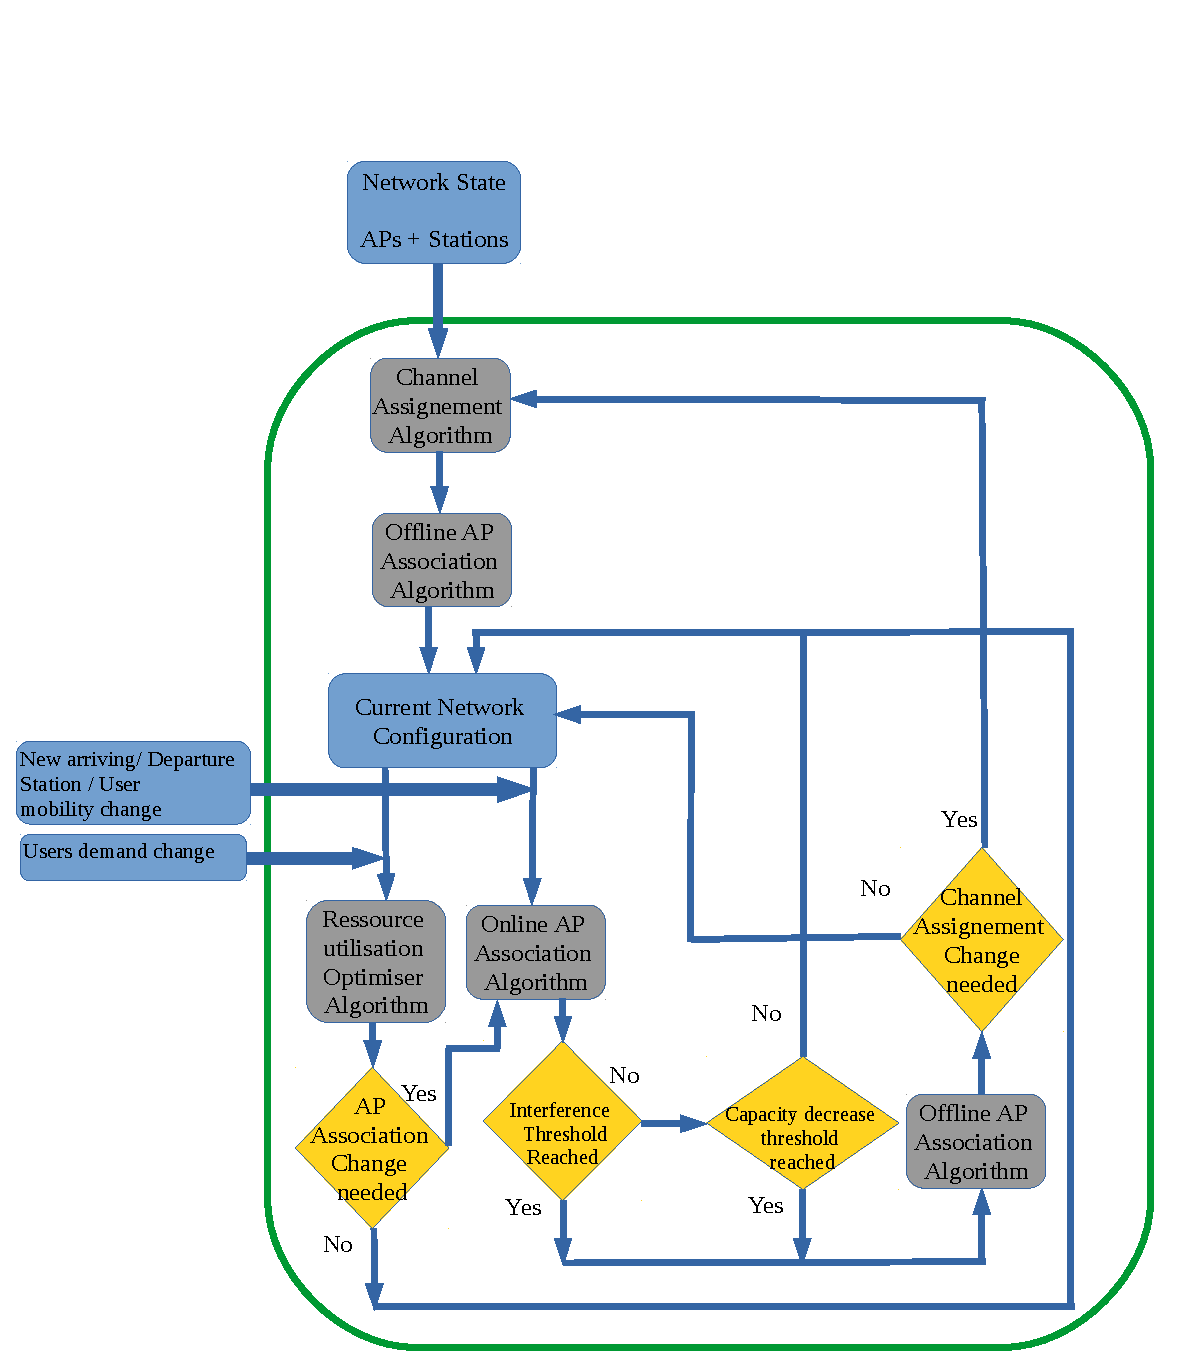
\includegraphics[width=9.cm]{Figures/diagramme_controler_functioning.pdf}
\caption{Complete Scheme for Radio Resource Management Interaction}
\label{fig:complete_RRM_scheme}
\end{figure}
%==============================================


\section{Conclusion} (me)
\label{Conclusion}
With the continuous and dense use of WLAN, experience has shown that standard association using 802.11 proofs some throughput limitations. In this study, we defined the important parts of Radio Ressource Management for WLAN. We focused afterthat on reviewing many works dealing with client Access Point Association as an important part for RRM. In fact, with the densification of users in WLAN scenarios from one hand, and the huge and differentiated resources demand according to the applications on the other hand, planning optimal association will bring better throughput to the users and load balance the Access Points charge. A deep discussion and classification thorough the paper highlighted the shortcoming of some proposed methods according to high applications requirements. The use of SDN paradigm for the controllers of WLAN was also discussed and its advantages described. For our future study, we plan to describe deeply the other RRM parts to allowing a complete comprehension of WLAN resources monitoring.      



\bibliographystyle{IEEEtran}
\bibliography{survey_wifi_controlers.bib}
\end{document}


\grid
